\documentclass{article}

\textwidth=125mm
\textheight=200mm
\linespread{1.04}


\title{\textsc{ExpByOpt for Convex Bandits}}
\usepackage{cancel}
\usepackage{marginnote}
\reversemarginpar % switch default margin to the left
\usepackage{bbm}
\usepackage{framed}
\usepackage{xcolor}
\usepackage{nicefrac}
\usepackage{pgfplots}
\pgfplotsset{compat=1.18}
\usepackage{floatrow}
\usepackage{amsmath}
\usepackage{amsthm}
\usepackage{listings}
\usepackage{tikz}
\usepackage{amssymb}
\usepackage[plain]{algorithm}
\lstset{emph={try,catch,throw,def,or,to,for,then,end,for,if,args,else,return},emphstyle=\color{blue!100!black}\bfseries}
\lstset{mathescape=true,escapechar=\&,numbers=left,xleftmargin=3mm,linewidth=0.47\textwidth,framextopmargin=0pt,framexbottommargin=0pt,aboveskip=-1pt,belowskip=-1pt}
\usepackage{mdframed}
\usepackage{bm}
\usepackage[bf]{caption}
\usepackage{graphicx}
\usepackage{xspace}
\usepackage{mathtools}
\usepackage{natbib}
\usepackage{hyperref} % add backlinks to the end of bibliography items
\usepackage[capitalise]{cleveref}

\definecolor{dkblue}{cmyk}{1,.54,.04,.19} 
\theoremstyle{plain}
\newtheorem{theorem}{Theorem}
\newtheorem{optprob}[theorem]{Optimisation Problem}
\newtheorem{lemma}[theorem]{Lemma}
\newtheorem{proposition}[theorem]{Proposition}
\newtheorem{corollary}[theorem]{Corollary}
\newtheorem{claim}[theorem]{Claim}
\theoremstyle{definition}
\newtheorem{definition}[theorem]{Definition}
\newtheorem{example}[theorem]{Example}
\newtheorem{remark}[theorem]{Remark}
\newtheorem{question}[theorem]{Question}
\newtheorem{fact}[theorem]{Fact}
\newtheorem{assumption}[theorem]{Assumption}

\renewcommand{\P}{\mathbb{P}}
\renewcommand{\epsilon}{\varepsilon}
\newcommand{\ind}[1]{^{{\scriptscriptstyle(#1)}}}
\newcommand{\reason}[1]{\texttt{(#1)}}
\newcommand{\by}[2]{\stackrel{\texttt{(#1)}}{#2}}
\newcommand{\half}{\tfrac{1}{2}}
\newcommand{\pr}{\texttt{pr}}
\newcommand{\po}{\texttt{po}}
\newcommand{\dom}[1]{\operatorname{dom}(#1)}
\newcommand{\dA}{\tilde{A}}
\newcommand{\cN}{\mathcal{N}}
\newcommand{\cM}{\mathcal{M}}
\newcommand{\cB}{\mathcal{B}}
\newcommand{\cR}{\mathcal{R}}
\newcommand{\cV}{\mathcal{V}}
\newcommand{\alg}{\mathcal{A}lg}
\newcommand{\ceil}[1]{\left\lceil #1 \right\rceil}
\newcommand{\R}{\mathbb R}
\newcommand{\Rd}{\mathbb{R}^d}
\newcommand{\argmin}{\operatornamewithlimits{arg\,min}}
\newcommand{\argmax}{\operatornamewithlimits{arg\,max}}
\newcommand{\ip}[1]{\langle #1 \rangle}
\newcommand{\Reg}{\mathfrak{R}}
\newcommand{\BReg}{\mathfrak{BR}}
\newcommand{\norm}[1]{\Vert #1 \Vert}
\newcommand{\E}{\mathbb E}
\newcommand{\Var}{\operatorname{Var}}
\newcommand{\Cov}{\operatorname{Cov}}
\newcommand{\cE}{\mathcal E}
\newcommand{\cK}{\mathcal K}
\newcommand{\cH}{\mathcal H}
\newcommand{\cT}{\mathcal T}
\newcommand{\cF}{\mathcal F}
\newcommand{\cO}{\mathcal O}
\newcommand{\cS}{\mathcal S}
\newcommand{\cC}{\mathcal C}
\newcommand{\cL}{\mathcal L}
\newcommand{\cG}{\mathcal G}
\newcommand{\cA}{\mathcal A}
\newcommand{\cD}{\mathcal D}
\newcommand{\cP}{\mathcal P}
\newcommand{\BS}{\mathbb S}
\newcommand{\zeros}{ \bm 0}
\newcommand{\polylog}{\operatorname{polylog}}
\newcommand{\const}{\operatorname{const}}
\newcommand{\interior}{\operatorname{int}}
\newcommand{\conv}{\operatorname{conv}}
\newcommand{\diam}{\operatorname{diam}}
\renewcommand{\d}[1]{\operatorname{d}\!#1}
\newcommand{\abovelabel}[1]{\stackrel{\raisebox{0.5mm}{\textrm{\tiny \color{red} #1}}}}
\newcommand{\ta}{\tilde{a}}
\newcommand{\tP}{P'}
\newcommand{\tA}{A'}
\newcommand{\fmd}{\texttt{MD}}
\newcommand{\tfmd}{\widetilde{\texttt{MD}}}

\newcommand{\mdalg}{\textsf{MD}\xspace}
\newcommand{\smdalg}{\textsf{SMD}\xspace}
\newcommand{\expbyopt}{\textsf{ExpByOpt}\xspace}
\newcommand{\expthree}{\textsf{Exp3}\xspace}
\newcommand{\expthreeix}{\textsf{Exp3.IX}\xspace}
\newcommand{\olo}{\texttt{OLO}\xspace}
\newcommand{\blo}{\texttt{BLO}\xspace}
\newcommand{\bco}{\texttt{BCO}\xspace}
\newcommand{\oco}{\texttt{OCO}\xspace}
\newcommand{\hl}{\hat{\ell}\xspace}


\begin{document}
\maketitle

\section{Overview}
In this note, we aim to improve the dimension dependence of bandit convex optimization (\bco).
The main theoretical tool we use is mirror descent (\mdalg).
We start by reviewing online linear optimization (\olo) and bandit linear optimization (\blo).
Then we move on to \bco.
The current state of affairs can be summarized as follows:
\begin{enumerate}
    \item \oco reduces to \olo: $f(x) - f(x_\star) \leq \langle f'(x), x - x_\star \rangle$.
    \item \textbf{Random} algs are \textit{suboptimal} for \texttt{OCO} and \textit{pointless} for \texttt{OLO}.
    \item First order information $f'(x)$ makes \texttt{BCO} as hard as \texttt{OLO}.
    \item \textbf{Random} algs are \textit{necessary} for \texttt{BCO} and \texttt{BLO}.
    \item \textbf{Random} algs are \textit{free} for \texttt{BLO} but appear to be \textit{expensive} ($d^{1.5}$) for \texttt{BCO}.
\end{enumerate}
\subsection{Notation}
Let $[n] = \{1,2, \cdots, n\}$.
Let $D_F(a, b) = F(a) - F(b) - F'(b)^\top (a - b)$ be the Bregman divergence.
Also let $\cP(A)$ be the set of all probability measures over the set $A$,
equipped with appropriate $\sigma$-algebra.
We use uppercase letters such as $A, B, X, Y$ to denote random variables or elements.

Let $\interior(\cD)$ be the interior of the set $\cD$.
For a convex function $F: \Rd \to \R \cup \{+\infty\}$
let $\dom{F} = \{x \in \Rd: F(x) < \infty\}$ be the domain of $F$.
A convex function $F$ is \emph{proper} if $\dom{F} \neq \emptyset$.
A convex function $F$ is \emph{closed} if its epigraph $\text{epi}(F) = \{(x, t) \in \Rd \times \R: F(x) \leq t\}$ is a closed set.
In this note, we only consider proper closed convex functions.

\section{Preliminaries: online optimization and regret}
Online optimization is a repeated game between a player and an adversary.
In each round $t \in [n]$, the player chooses an action $a_t$ from an action set $\cA$ (usually assumed to be convex and compact), and the adversary chooses a loss function $f_t: \cA \to \R$ from a class of functions $\cF$ (e.g., linear, convex, Lipschitz, smooth, etc.).
The player then incurs loss $f_t(a_t)$.
The regret w.r.t. an action $a_\star \in \cA$ is defined as
\begin{align*}
    \Reg_n(a_\star) = \sum_{t=1}^{n} f_t(a_t) - f_t(a_\star)\,.
\end{align*}
The adversary is free to choose $f_t$ adaptively based on the player's past actions $a_1, \cdots, a_{t-1}$.
The player is allowed to randomize its actions, i.e., $A_t$ can be a random element taking values in $\cA$.
Then the expected regret is defined as
\begin{align*}
    \E[\Reg_n(a_\star)] = \E\left[\sum_{t=1}^{n} f_t(A_t) - f_t(a_\star)\right]\,,
\end{align*}
where the expectation is taken w.r.t. the randomness of the player's actions (and the induced randomness in $f_t$ if the adversary is adaptive).
The goal is to minimize the expected regret uniformly over all possible sequences of losses and all actions $a_\star \in \cA$.

In the \textit{full-information} setting, at the end of each round $t \in [n]$,
the player observes the entire loss function $f_t$.
In the \textit{bandit} setting, the player only observes the incurred loss $f_t(a_t)$.
We will study both settings in the following sections.

\section{Online linear optimization (\texttt{OLO})}
By online linear optimization, we mean the following \textit{full-information} game between a player and an adversary, where the losses $f_t$ are linear functions.
Since $f_t$ is linear, we can write $f_t(a) = \langle \ell_t, a \rangle$ for some loss vector $\ell_t \in \Rd$.
Then, the regret w.r.t. an action $a_\star \in \cA$ is defined as
\begin{align*}
    \Reg_n(a_\star) = \sum_{t=1}^{n} \langle \ell_t, a_t - a_\star \rangle\,.
\end{align*}
The algorithm we study for \olo is mirror descent (\mdalg),
which is presented in \cref{alg:MD}.

\begin{mdframed}
    \begin{definition}[Legendre function]
        A convex function $F$ is called \emph{Legendre} if:
        \begin{enumerate}
            \item $\interior(\dom{F})$ is nonempty;
            \item $F$ is strictly convex on $\interior(\dom{F})$;
            \item $F$ is differentiable on $\interior(\dom{F})$;
            \item if $x_n\to x\in\partial\dom{F}$ then $\|F'(x_n)\|\to\infty$.
        \end{enumerate}
    \end{definition}
\end{mdframed}

Suppose that $\cA \subset \Rd$ is convex and compact,
and $F: \Rd \to \R \cup \{+\infty\}$ is a Legendre function such that $\cA \cap \interior(\dom{F}) \neq \emptyset$.


For a sequence of losses $\ell_{1:t-1}$, we define the functions $\fmd(\ell_{1:t-1})$
and $\tfmd(\ell_{1:t-1})$ to be the actions $a_t$ and $\ta_t$
in \cref{alg:MD}, when the loss sequence $\ell_{1:t-1}$ is fed to the algorithm.
\begin{algorithm}[h!]
    \begin{minipage}{12cm}
        \begin{mdframed}
            \begin{lstlisting}
args: $\eta > 0$, potential function $F$
$a_1 = \argmin_{a \in \cA} F(a)$
for $t = 1$ to $n$:
    Play $a_t$ and observe $\ell_t$
    $\ta_{t+1} = \argmin_{a \in \Rd} \eta \langle a, \ell_t\rangle + D_F(a, a_t)$
    $a_{t+1} = \argmin_{a \in \cA} D_F(a, \ta_{t+1})$
\end{lstlisting}
            \caption{\mdalg---
                It also holds that $a_{t+1} = \argmin_{a \in \cA} \eta \langle a, \ell_t\rangle + D_F(a, a_t)$.
            }\label{alg:MD}
        \end{mdframed}
    \end{minipage}
\end{algorithm}
\begin{theorem}\label{thm:MD}
    Let $F$ be Legendre with domain $\cD$ such that $\cA \cap \interior(\cD)\neq \emptyset$.
    Then
    \begin{align*}
        \Reg_n(a_\star)
         & \leq
        \sum_{t=1}^{n} \langle \ell_t, a_t - a_{t+1} \rangle
        + \frac{1}{\eta}
        \left(
        D_F(a_\star, a_1) -
        \sum_{t=1}^{n} D_F(a_{t+1}, a_t)
        \right) \\
         & \leq
        \frac{1}{\eta}
        \left(
        D_F(a_\star, a_1) + \sum_{t=1}^{n} D_F(a_{t}, \tilde{a}_{t+1})
        \right).
    \end{align*}
    Moreover,
    $ D_F(a_{t}, \tilde{a}_{t+1})
        = D_{F^\star}\left(F'(a_t) - \eta \ell_t, F'(a_t)\right)$.
\end{theorem}
\begin{proof}
    We have
    \begin{align*}
        \Reg_n(a_\star)
         & = \sum_{t=1}^{n} \langle \ell_t, a_t - a_\star \rangle                                                                                                                                                                         \\
         & = \sum_{t=1}^{n} \underbrace{\langle \ell_t, a_t - a_{t+1} \rangle}_{\triangleq \texttt{st}_t \text{ or stability}} + \underbrace{\langle \ell_t, a_{t+1} - a_\star \rangle}_{\triangleq \texttt{tr}_t \text{ or tracking}}\,.
    \end{align*}
    What do we know about $a_{t+1}$?
    \begin{align*}
                    & a_{t+1} = \argmin_{a \in \cA} \eta \langle \ell_t, a \rangle + D_F(a, a_t)                                                                \\
        \Rightarrow &
        \forall \tilde{a} \in \cA, \quad
        \langle \eta \ell_t + F'(a_{t+1}) - F'(a_t), \tilde{a} - a_{t+1} \rangle \geq 0                                                                         \\
        \Rightarrow
                    & \texttt{tr}_t = \langle \ell_t, a_{t+1} - a_\star \rangle \leq \frac{1}{\eta} \langle F'(a_{t+1}) - F'(a_t), a_\star - a_{t+1} \rangle\,.
    \end{align*}
    Then there's the nice equality
    \begin{align*}
        \langle F'(a_{t+1}) - F'(a_t), a_\star - a_{t+1} \rangle
         & =
        D_F(a_\star, a_t) - D_F(a_{t+1}, a_t) - D_F(a_\star, a_{t+1})\,,
    \end{align*}
    which gives us a bound on the \textit{tracking} terms
    \begin{align*}
        \eta \sum_{t=1}^{n} \langle \ell_t, a_{t+1} - a_\star \rangle
         & \leq \sum_{t=1}^{n} D_F(a_\star, a_t)  - D_F(a_\star, a_{t+1}) - D_F(a_{t+1}, a_t)                   \\
         & = D_F(a_\star, a_1) - \underbrace{D_F(a_\star, a_{n+1})}_{\geq 0} - \sum_{t=1}^{n} D_F(a_{t+1}, a_t) \\
         & \leq D_F(a_\star, a_1) - \sum_{t=1}^{n} D_F(a_{t+1}, a_t)\,.
    \end{align*}
    Note that the tracking term scales inversely with $\eta$ as expected.
    Without touching the stability term, we have proved the first inequality,
    \begin{align*}
        \Reg_n(a_\star)
         & \leq
        \sum_{t=1}^{n} \langle \ell_t, a_t - a_{t+1} \rangle
        + \frac{1}{\eta}
        \left(
        D_F(a_\star, a_1) -
        \sum_{t=1}^{n} D_F(a_{t+1}, a_t)
        \right)\,.
    \end{align*}
    Next, we move onto the stability term.
    $\textsf{MD}$ stores the latest loss in the gradient of $\tilde{a}_{t+1}$,
    \begin{align*}
         & \tilde{a}_{t+1}  = \argmin_{a \in \R^d} \eta \langle \ell_t, a \rangle + D_F(a, a_t) \\
        \Rightarrow
         & \ell_t = \frac{1}{\eta}
        \left(
        F'(a_t) - F'(\tilde{a}_{t+1})
        \right)
    \end{align*}
    which results in another nice equality
    \begin{align*}
        \texttt{st}_t
         & = \langle \ell_t, a_{t} - a_{t+1} \rangle                                                                      \\
         & = \frac{1}{\eta} \langle F'(a_t) - F'(\tilde{a}_{t+1}), a_t - a_{t+1} \rangle                                  \\
         & = \frac{1}{\eta} \left(D_F(a_{t+1}, a_t) + D_F(a_t, \tilde{a}_{t+1}) - D_F(a_{t+1}, \tilde{a}_{t+1})\right)\,.
    \end{align*}
    Thus, by dropping the negative term $- D_F(a_{t+1}, \tilde{a}_{t+1})$,
    we have proved the second inequality,
    \begin{align*}
        \Reg_n(a_\star)
         & \leq
        \frac{1}{\eta}
        \left(
        D_F(a_\star, a_1) + \sum_{t=1}^{n} D_F(a_{t}, \tilde{a}_{t+1})
        \right)\,.
    \end{align*}
    To see the last part of the theorem, we use the definition of Bregman divergence
    \begin{align*}
        D_F(a_{t}, \tilde{a}_{t+1})
         & =D_{F^\star}\left(F'(\tilde{a}_{t+1}), F'(a_t)\right)       \\
         & = D_{F^\star}\left(F'(a_t) - \eta \ell_t, F'(a_t)\right)\,.
    \end{align*}
\end{proof}
\begin{remark}
    \label{rem:ellt-adapted}
    The analysis is remarkably amenable to different modifications.
    For instance, the result continues to work even if $\ell_t$ is adapted to $a_1, \cdots, a_{t-1}$---equivalently, $\ell_t$ is chosen adaptively by an adversary.
    Much of what comes after hinges on the generality of the proof of this theorem.
\end{remark}

\subsection*{When \texorpdfstring{$\cA=\Delta(d)$}{A=Delta(d)} and \texorpdfstring{$F$}{F} is the negentropy}\label{sec:md-negentropy}
The case that $\cA = \Delta(d)$ is the simplex and the potential
is negentropy,
\begin{align*}
    R(p) = \begin{cases}
               \langle p, \ln(p) - 1 \rangle & p \in \Rd_+    \\
               \infty                        & p \notin \Rd_+ \\
           \end{cases}
\end{align*}
is of special interest as it results in a sort of universal algorithm for all
action sets as long as they have a covering---the learner
can come up with the cover $\cA$ and randomize over that.
That being said, while being theoretically interesting, such an algorithm
would be computationally expensive as the size of the cover grows.

Note that $D_R = D_{KL}$, $R^\star(q) = \langle \exp(q), 1\rangle$,
$R'(p) = \ln(p)$, and ${R^\star}'(q) = \exp(q)$.
\begin{theorem}[\mdalg on simplex]\label{thm:md-simplex}
    Suppose that $\ell_t \in [0,1]^d$ and $\cA = \Delta(d)$.
    Then the regret of \mdalg with $R$ as the potential
    with learning rate $\eta \in (0,1]$
    satisfies
    \begin{align*}
        \Reg_n(a_\star) \leq
        \frac{\ln(d)}{\eta}
        +
        \eta\sum_{t=1}^{n} \langle a_t, \ell_t^2\rangle
        \leq 2 \sqrt{n\ln(d)}\,.
    \end{align*}
\end{theorem}
\begin{proof}
    From theorem~\ref{thm:MD}, we have
    \begin{align*}
        \Reg_n(a_\star)
         & \leq
        \frac{1}{\eta}
        \left(
        D_R(a_\star, a_1) + \sum_{t=1}^{n} D_{R^\star}\left(R'(a_t) - \eta \ell_t, R'(a_t)\right)
        \right)
        \\
         & \leq
        \frac{1}{\eta}
        \left(
        \ln(d) + \sum_{t=1}^{n} R^\star(R'(a_t) - \eta \ell_t) - R^\star(R'(a_t)) - a_t^\top(-\eta \ell_t)
        \right)
        \\
         & =
        \frac{1}{\eta}
        \left(
        \ln(d) + \sum_{t=1}^{n} \langle \exp(\ln(a_t) - \eta \ell_t) - \exp(\ln(a_t)), 1 \rangle + \langle a_t, \eta \ell_t\rangle
        \right)
        \\
         & =
        \frac{1}{\eta}
        \left(
        \ln(d) + \sum_{t=1}^{n} \langle a_t, \exp(- \eta \ell_t) - 1 \rangle + \langle a_t, \eta \ell_t\rangle
        \right)
        \\
         &
        \abovelabel{$\eta \|\ell_t\|_\infty \leq 1$}
        \leq
        \frac{1}{\eta}
        \left(
        \ln(d) + \sum_{t=1}^{n} \langle a_t, 1 - \eta \ell_t + \eta^2 \ell_t^2 - 1 \rangle + \langle a_t, \eta \ell_t\rangle
        \right)
        \\
         &
        =
        \frac{1}{\eta}
        \left(
        \ln(d) + \eta^2\sum_{t=1}^{n} \langle a_t, \ell_t^2\rangle
        \right)\,.
    \end{align*}
    In order to get a bound in terms of $d$ and $n$,
    we use the fact that $\ell_t \in [0,1]^d$ to get
    \begin{align*}
        \Reg_n(a_\star) & \leq
        \frac{\ln(d)}{\eta}
        +
        \eta\sum_{t=1}^{n} \langle a_t, \ell_t^2\rangle \\
                        & \leq
        \frac{\ln(d)}{\eta}
        +
        \eta \sum_{t=1}^{n} \|a_t\|_1 \|\ell_t^2\|_\infty
        \\
                        & \leq
        \frac{\ln(d)}{\eta}
        +
        \eta n
        \leq 2 \sqrt{n\ln(d)}\,.
    \end{align*}
    The better bound of $\sqrt{2n\ln(d)}$ is also possible by using
    $\exp(-x) \leq 1 - x + \frac{x^2}{2}$.
\end{proof}

\section{Bandit linear optimization (\blo)}
In the bandit setting, the learner only observes $y_t = \langle \ell_t, a_t \rangle$, instead of $\ell_t$.

\paragraph{The need for randomization:}
In the bandit setting, it is necessary for the learner to randomize its actions,
as shown by the next theorem.
\begin{theorem}[Failure of determinism in bandit feedback]
    \label{thm:blo-deterministic}
    Consider \blo with action set $\cA=\Delta(2)$, and loss vectors $\ell_t \in [0,1]^2$.
    The loss of playing $p_t\in\Delta(2)$ is $\langle \ell_t, p_t\rangle$.
    Then, for every deterministic algorithm and every horizon $n$,
    there exists a loss sequence $(\ell_t)_{t=1}^n\subset[0,1]^2$
    such that the regret satisfies
    \[
        \max_{p\in\Delta(2)} \sum_{t=1}^{n}\langle \ell_t, p_t - p \rangle \;\ge\; \frac{n}{4}.
    \]
\end{theorem}
\begin{proof}
    We only provide the proof sketch here.
    The idea is to only show $1/2$ loss to the learner in each round,
    and observe its action $p_t$.
    Let $a_t$ be the second coordinate of $p_t$.
    WLOG, assume that $a_t \geq 1/2$ for at least $n/2$ rounds.
    Then, in those rounds, the adversary sets $\ell_t = (0,\frac{1}{2 a_t})$,
    resulting in loss $1/2$ to the learner (since $\langle \ell_t, p_t \rangle = a_t \cdot \frac{1}{2 a_t} = 1/2$).
    In the other rounds, the adversary sets $\ell_t = (\frac{1}{2},\frac{1}{2})$.
    Thus, the learner suffers the loss of $1/2$ in each round that it plays $a_t \geq 1/2$,
    compared to the $p_\star = (1,0)$ which suffers zero loss in those rounds.
    Therefore, in total, the learner suffers at least $n/4$ regret.
\end{proof}


\subsection{Stochastic mirror descent(\smdalg)}
\begin{algorithm}[h!]
    \begin{minipage}{12cm}
        \begin{mdframed}
            \begin{lstlisting}
args: $\eta > 0$, potential function $F$
$a_1 = \argmin_{a \in \cA} F(a)$
$\ta_1 = \argmin_{a \in \Rd} F(a)$
for $t = 1$ to $n$:
    Choose $P_t \in \cP(\cA)$, s.t. $\E_{A \sim P_t}[A] = a_t$
    Choose $E_t: \cA \times \R \to \Rd$
    Play $A_t \sim P_t$ and observe $Y_t=\langle A_t, \ell_t \rangle$
    Compute $\hl_t = E_t(A_t, Y_t)$
    $a_{t+1} = \argmin_{a \in \cA} \eta \langle a, \hl_t\rangle + D_F(a, a_t)$
    $\ta_{t+1} = \argmin_{a \in \Rd} \eta \langle a, \hl_t\rangle + D_F(a, \ta_t)$
\end{lstlisting}
            \caption{\smdalg}\label{alg:SMD}
        \end{mdframed}
    \end{minipage}
\end{algorithm}

\marginnote{\textit{Exploration is free in \blo}}
Instead of choosing an action $a_t \in \cA$, \smdalg chooses an
\textit{exploration} distribution $P_t \in \cP(\cA)$
\textbf{with mean} $a_t$ in round $t \in [n]$.
Since losses are linear in {\blo}, we have that
\begin{align*}
    \E[\langle A_t, \ell_t \rangle] = \langle a_t, \ell_t\rangle\,,
\end{align*}
which means \smdalg and \mdalg have the \textbf{same expected loss} given
the \mdalg action $a_t$.

\marginnote{\textit{$\hl$ vs $\ell$}}
The issue is that \smdalg does not observe $\ell_t$.
Instead, \smdalg pretends that $\hl_t$ which is an \textit{estimate} of $\ell_t$ is the actual loss.
\textbf{In the most general form}, this estimation can be made through a function
$E_t: \cA \times \R \to \Rd$ in each round $t \in [n]$ such that $\hl_t = E_t(A_t, Y_t)$.
\begin{theorem}[Unbiased-\smdalg]\label{thm:SMD-unbiased}
    Suppose $\E[\hl_t|\fmd(\hl_{1:t-1})] = \ell_t$ (unbiased estimator).
    The regret of $\smdalg$ is bounded as
    \begin{align*}
        \Reg_n(a_\star)
         & \leq
        \frac{D_F(a_\star, a_1)}{\eta}
        +
        \E\left[
            \sum_{t=1}^{n}
            \left(
            \langle \hl_t, \fmd(\hl_{1:t-1}) - \fmd(\hl_{1:t}) \rangle
            - \frac{1}{\eta}
            D_F(\fmd(\hl_{1:t-1}), \fmd(\hl_{1:t}))
            \right)
        \right] \\
         & \leq
        \frac{1}{\eta}\left(
        D_F(a_\star, a_1)
        +
        \E\left[
            \sum_{t=1}^{n} D_F(\fmd(\hl_{1:t-1}), \tfmd(\hl_{1:t}))
            \right]
        \right)\,.
    \end{align*}
\end{theorem}
\begin{proof}
    The proof follows simply from
    \begin{align*}
        \Reg_n(a_\star)
        =
        \E\left[
            \sum_{t=1}^{n} \langle A_t - a_\star, \ell_t\rangle
            \right]
        =
        \E\left[
            \sum_{t=1}^{n} \langle \fmd(\hl_{1:t-1}) - a_\star, \hl_t\rangle
            \right]\,,
    \end{align*}
    and applying theorem~\ref{thm:MD} to the random game inside the expectation.

    Note that $\hl_t$ is adapted to $a_1, \cdots, a_{t-1}$, but as stated in
    remark~\ref{rem:ellt-adapted}, the analysis of theorem~\ref{thm:MD}
    continues to hold in this case.
\end{proof}


\subsubsection{Unbiased estimation with one sample}
In \cref{thm:SMD-unbiased}, we assumed that $\hl_t$ is an unbiased estimator of $\ell_t$.
However, it is not clear if it is possible to construct such an estimator
with one sample $Y_t = \langle A_t, \ell_t \rangle$.
However, the next lemma not only shows that such a task is possible,
but also shows that it is possible for whole classes of distributions
$P_t$ with invertible second moment matrix.
\begin{lemma}[Unbiased 1-sample estimator]
    \label{lem:1-sample-estimator}
    Let $v \in \R^d$ be a vector,
    and $P \in \cP(\Rd)$ be a distribution.
    There exists a function $E: \Rd \times \R \to \Rd$ such that
    \begin{align*}
        \E_{A \sim P}[E(A, \langle A, v \rangle)] = v\,,
    \end{align*}
    if $\E_{A \sim P}[A A^\top]$ is invertible.
\end{lemma}
\begin{proof}
    Let $Y = \langle A, v \rangle$.
    It suffices to use
    \begin{align*}
        E(a, y) = \E_{A \sim P}[A A^\top]^{-1} a  y\,.
    \end{align*}
    This ensures that
    \begin{align*}
        \E_{A \sim P}[E(A, \langle A, v \rangle)]
         & = \E_{A \sim P}[\E_{A \sim P}[A A^\top]^{-1} A  \langle A, v \rangle] \\
         & = \E_{A \sim P}[A A^\top]^{-1} \E_{A \sim P}[A  A^\top v]             \\
         & = \E_{A \sim P}[A A^\top]^{-1} \E_{A \sim P}[A A^\top]  v             \\
         & = v\,.
    \end{align*}
\end{proof}
This shows that as long as the second moment matrix of $P_t$ is invertible,
it is possible to construct a sequence of unbiased estimators $\hl_t$,
such that $\E_t[\hl_t] = \ell_t$.

\subsubsection{Biased \smdalg}
\begin{algorithm}[h!]
    \begin{minipage}{13cm}
        \begin{mdframed}
            \begin{lstlisting}
args: $\eta > 0$, potential function $F$
$a_1 = \argmin_{a \in \cA} F(a)$
$\ta_1 = \argmin_{a \in \Rd} F(a)$
for $t = 1$ to $n$:
    Choose $P_t \in \cP(\cA)$ and $E_t \in (\Rd)^{(\cA \times \R)}$, as functions of $a_t$.
    Play $A_t \sim P_t$ and observe $Y_t = \langle A_t, \ell_t\rangle$
    Compute $\hl_t = E_t(A_t, Y_t)$
    $a_{t+1} = \argmin_{a \in \cA} \eta \langle a, \hl_t\rangle + D_F(a, a_t)$
\end{lstlisting}
            \caption{Biased \smdalg}\label{alg:biased-SMD}
        \end{mdframed}
    \end{minipage}
\end{algorithm}

Suppose there are two sampling rules $P_t, P_t' \in \cP(\cA)$ where
$\E_{A \sim P_t}[A] = \E_{A \sim P_t'}[A]$, and \smdalg should choose
one of them for sampling $A_t$ at round $t$.
In \blo, these two \textit{result in the exact same loss} in round $t$,
so how to choose between them?
If one is biased and the other is unbiased,
is the unbiased one always preferred?
The answer seems to be \textit{no}: compare the \expthree and \expthreeix algorithms.

For the moment, we formulate this question.
We define a variant of \smdalg where $P_t$ and $E_t$
can be chosen freely as long as they are functions of $a_t$.
We call this variant Biased-\smdalg and present it in \cref{alg:biased-SMD}.
\begin{remark}[Is this an \mdalg-type of algorithm anymore?]
    At this point, it is fair to ask in what sense this is related
    to \mdalg? The key that distinguish Biased-\smdalg from
    \textit{all possible algorithms} is that $P_t$ and $E_t$
    are only functions of $a_t$ in Biased-\smdalg.
\end{remark}

\begin{theorem}[Biased-\smdalg, (\cite{lattimore2024bandit}, Theorem 8.14)]\label{thm:SMD-biased}
    The expected regret of Biased-\smdalg is bounded by
    \begin{align*}
        \frac{D_F(a_\star, a_1)}{\eta} +
        \sum_{t=1}^{n}
        \E\left[
            \langle A_t - a_\star, \ell_t\rangle
            - \langle \hat{a}_t - a_\star, \hl_t\rangle
            + \frac{1}{\eta} D_{F^\star}(F'(\hat{a}_t) - \eta \hl_t, F'(\hat{a}_t))
            \right]\,.
    \end{align*}
    where $\hat{a}_t = \fmd(\hl_{1:t-1})$.
\end{theorem}
\begin{proof}
    We have
    \begin{align*}
         & \Reg_n(a_\star)
        =
        \E\left[
            \sum_{t=1}^{n}
            \langle A_t - a_\star, \ell_t\rangle
        \right]            \\
         & =
        \E\left[
            \sum_{t=1}^{n}
            \langle A_t - a_\star, \ell_t\rangle
            - \langle \hat{a}_t - a_\star, \hl_t\rangle
            + \langle \hat{a}_t - a_\star, \hl_t\rangle
            \right]
        \\
         & \leq
        \E\left[
            \frac{D_F(a_\star, \hat{a}_1)}{\eta}
            +
            \sum_{t=1}^{n}
            \langle A_t - a_\star, \ell_t\rangle
            - \langle \hat{a}_t - a_\star, \hl_t\rangle
            + \frac{1}{\eta} D_{F^\star}(F'(\hat{a}_t) - \eta \hl_t, F'(\hat{a}_t))
            \right]\,,
    \end{align*}
    where the inequality is by theorem~\ref{thm:MD}.
    Also note that $\hat{a}_1 = a_1$ since $\hl_{1:0}$ is an empty sequence.
\end{proof}
\begin{remark}[\fmd{} in a virtual game]
    Note that $\hl_t$ is adapted to $A_t$ since the algorithm actually plays
    $A_t \sim P_t$.
    So you can think that $P_t$ is the exploration policy that
    is actually played which is not \smdalg as
    $\E[A_t|\fmd(\hl_{1:t-1})] \neq \fmd(\hl_{1:t-1})$.
    However, in the analysis we suppose that $\fmd(\hl_{1:t-1})$ is played
    \textbf{without any randomization} (so technically \mdalg) on
    $\hl_1, \cdots, \hl_n$.
\end{remark}

\begin{remark}[Closer look at theorem~\ref{thm:SMD-biased}---a dummy bound]
    \label{rem:dummy-bound}
    If we look closer at theorem~\ref{thm:SMD-biased}, we can see that
    $\sum_{t=1}^{n} \E[\langle A_t - a_\star, \ell_t\rangle]$ term
    that appears on the RHS of the claim is exactly $\Reg_n(a_\star)$,
    so we did bound $\Reg_n(a_\star)$ by $\Reg_n(a_\star) + \square$ and
    for this theorem to be useful this $\square$ better be negative.
    More precisely, we did nothing other than adding and subtracting the value of the game
    that is played on $\hl_{1:n}$: the algorithm is \mdalg (not {\smdalg})
    and the loss sequence is $\hl_{1:n}$.
    So if we show the value of this game by $\hat{G}_n$, all we did is
    \begin{align*}
        \Reg_n(a_\star) = \Reg_n(a_\star) - \hat{G}_n + \hat{G}_n \,,
    \end{align*}
    which is an equality so far.
    The inequality is there for two reasons: (1) the upper-bound on
    $+ \hat{G}_n$, which is \textit{unavoidable},
    (2) $a_\star \neq \hat{a}_\star$---the true minimizer of the
    \textit{estimated game sequence} $\hl_{1:n}$ is not necessarily
    $a_\star$.
    The second reason might actually make the $\square$ term positive
    and the theorem useless.
    Needless to say, the theorem still holds if we exchange $a_\star$
    for $\hat{a}_\star$.
\end{remark}

In the next section, we present a particular way of choosing $P_t$ and $E_t$
that results in a low-regret algorithm.

\section{Exploration By Optimization(\expbyopt)}
The idea is to choose $P_t$ and $E_t$ in each round $t \in [n]$
to minimize the term inside the expectation in theorem~\ref{thm:SMD-biased}
which is
\begin{align*}
    \E\left[
        \langle A_t - a_\star, \ell_t\rangle
        - \langle \hat{a}_t - a_\star, \hl_t\rangle
        + \frac{1}{\eta} D_{F^\star}(F'(\hat{a}_t) - \eta \hl_t, F'(\hat{a}_t))
        \right]\,.
\end{align*}
It's helpful to remind ourselves what is random here: $A_t \sim P_t$ and
$\hl_t = E_t(A_t, Y_t)$ where $Y_t = \langle A_t, \ell_t \rangle$,
so the \text{expectation is only over $A_t$}.

\begin{algorithm}[h!]
    \begin{minipage}{12cm}
        \begin{mdframed}
            \begin{lstlisting}
args: learning rate $\eta >0$, precision $\epsilon > 0$
for $t = 1$ to $n$:
    compute $a_t = \fmd(\hl_{1:t-1})$
    find distribution $P_t \in \cP(\cA)$ and $E_t \in (\Rd)^{(\cA \times \R)}$ s.t.
        $\sup_{\ell, a_\star} \Lambda_{a_t, \eta}(P_t, E_t) \leq \inf_{P,E} \sup_{\ell, a_\star} \Lambda_{a_t, \eta}(P, E) + \epsilon$
    sample $A_t \sim P_t$, and observe $Y_t = \langle \ell_t, A_t \rangle$
    compute $\hl_t = E_t(A_t, Y_t)$
\end{lstlisting}
            \caption{\expbyopt}\label{alg:exp-by-opt}
        \end{mdframed}
    \end{minipage}
\end{algorithm}

Perhaps more precisely, suppose it's round $t$; the learner knows what \mdalg suggests to play, i.e., $\hat{a}_t = \fmd(\hl_{1:t-1})$.
The idea is to choose the best $P_t$ and $E_t$ given $\hat{a}_t$,
hoping that the term inside the expectation in theorem~\ref{thm:SMD-biased} could
then be bounded uniformly for all $t \in [n]$.
To this end, with $A\sim P$ and
$\hl = E(A, Y) = E(A, \langle A, \ell\rangle)$, define
\begin{align}
    \label{eq:Lambda-original}
    \Lambda_{a, \eta}(P, E || a_\star, \ell) \triangleq
    \frac{1}{\eta}
    \E\left[
        \langle A - a_\star, \ell\rangle
        - \langle a - a_\star, \hl\rangle
        + \frac{1}{\eta} D_{F^\star}(F'(a) - \eta \hl, F'(a))
        \right]\,,
\end{align}
Then, a bound on
\begin{align*}
    \Lambda_{\cA, \cL, F}^\star \triangleq
    \sup_{\eta \geq 0, a \in \cA}
    \inf_{P \in \cP(\cA), E \in (\R^d)^{\cA \times \R}}
    \sup_{a_\star \in \cA, \ell \in \cL}
    \Lambda_{a, \eta}(P, E || a_\star, \ell)\,,
\end{align*}
will  result in a regret bound for \expbyopt.
\begin{theorem}[Regret of \expbyopt]
    \label{thm:exp-by-opt-regret}
    The expected regret of \expbyopt with precision $\epsilon > 0$
    is bounded as
    \begin{align*}
        \Reg_n(a_\star) \leq
        \inf_{\eta > 0}
        \left(
        \frac{D_F(a_\star, a_1)}{\eta}
        +
        n \eta
        \left(
            \Lambda_{\cA, \cL, F}^\star + \epsilon
            \right)
        \right)\,.
    \end{align*}
\end{theorem}
\begin{proof}
    The proof follows directly from theorem~\ref{thm:SMD-biased}
    and the definition of \expbyopt.
\end{proof}
Moreover, if we allow the second sup player to randomize, the resulting
saddle point value can't get smaller,
so let $\nu \in \cP(\cA \times \cL)$ and
\begin{align*}
    \Lambda_{a, \eta}(P, E || \nu) \triangleq
    \frac{1}{\eta}
    \E_{(A_\star, \ell) \sim \nu}\left[
        \langle A - A_\star, \ell\rangle
        - \langle a - A_\star, \hl\rangle
        + \frac{1}{\eta} D_{F^\star}(F'(a) - \eta \hl, F'(a))
        \right]\,,
\end{align*}
and note that
\begin{align*}
    \sup_{a_\star \in \cA, \ell \in \cL}
    \Lambda_{a, \eta}(P, E || a_\star, \ell)
    \leq
    \sup_{\nu \in \cP(\cA \times \cL)}
    \Lambda_{a, \eta}(P, E || \nu)\,.
\end{align*}
This change introduces convexity in the second player's strategy set,
which results in the following minimax theorem.
\begin{lemma}[\cite{lattimore2024bandit}, Lemma 8.21]
    \label{lem:exp-by-opt-minimax}
    For all $\eta > 0, a \in \cA$,  we have
    \begin{align*}
        \inf_{P \in \cP(\cA), E \in (\R^d)^{\cA \times \R}}
        \sup_{\nu \in \cP(\cA \times \cL)}
        \Lambda_{a,\eta}(P, E || \nu)
        =
        \sup_{\nu \in \cP(\cA \times \cL)}
        \inf_{P \in \cP(\cA), E \in (\R^d)^{\cA \times \R}}
        \Lambda_{a,\eta}(P, E || \nu)\,.
    \end{align*}
\end{lemma}
\begin{remark}
    The second $A_\star$ in $\Lambda(P, E || \nu)$
    can be switched with any fixed action $a \in \cA$.
    See remark~\ref{rem:dummy-bound}.
\end{remark}

\subsection{General estimators}
Let $\cP(\nu, P) = \E_{A \sim P, (A_\star, \ell) \sim \nu}\!\left[\langle A - A_\star, \ell \rangle\right]$.
The inf player can choose the best optimizer given the
$\nu$ choice of the adversary and its own sampling policy $P$.
\textbf{Most notably, we see that the optimal estimator doesn't depend on the choice of sampling policy $P$},
and following lemma shows that it comes with a closed form.
\begin{lemma}
    \label{lem:optimal-E}
    Given $\nu \in \cP(\cA \times \cL)$, and any $P \in \cP(\cA)$,
    there exists $G^\nu \in (\Rd)^{(\cA \times \R)}$ such that
    \begin{align*}
        G^\nu(b, y) & =
        \frac{1}{\eta}\left(
        F'(a) - F'(\E[A_\star|Y = y, A = b])
        \right)\,,
    \end{align*}
    and
    $
        \inf_{E \in (\Rd)^{\cA \times \R}}
        \Lambda(P, E || \nu)
        =
        \Lambda(P, G^\nu|| \nu)\,.
    $
\end{lemma}
\noindent The proof is deferred to \ref{proof:lem:optimal-E}.
For reasons that will be clear later, let
$\pr = \E[A_\star]$ (`pr' for prior) and
$\po = \E[A_\star|A, Y]$ (`po' for posterior).
\begin{lemma}
    \label{lem:optimal-Lambda-wrong-turn}
    When using the optimal estimator $G^\nu$, we have
    \begin{align*}
        \Lambda(P, G^\nu|| \nu)
         & = \frac{1}{\eta} \Delta(\nu, P)
        - \frac{1}{\eta^2}
        \E\!\left[
            D_F\left(\po, a\right)
            \right]\,.
    \end{align*}
\end{lemma}
\noindent The proof is deferred to \ref{proof:lem:optimal-Lambda-wrong-turn}.
Although the result of lemma~\ref{lem:optimal-Lambda-wrong-turn} is
elegant, it is not useful for proving the connection to the information ratio.
\begin{lemma}[Expected Bregman Identity]
    Let $F:\R^d \to \R$ be a strictly convex and differentiable function.
    For any random vector $X$ and any point $a$ in the domain of $F$, we have
    \begin{align*}
        \E\left[D_F(X, a)\right]
         & =
        \E\left[
            D_F\left( X, \E[X]\right)
            \right]
        +
        D_F\left( \E[X], a\right)
        \\
         & = \E[F(X)] - F(\E[X]) + D_F\left( \E[X], a\right).
    \end{align*}
\end{lemma}

\begin{lemma}
    \label{lem:the-right-turn}
    When using the optimal estimator $G^\nu$, we have
    \begin{align*}
        \E\left[D_F\left(\po, a\right)\right]
         & =
        \E\left[
            D_F\left( \po, \pr\right)
            \right]
        +
        D_F\left( \pr, a\right)\,.
    \end{align*}
\end{lemma}
\begin{proof}
    Follows directly from the expected Bregman identity and $\E[\po] = \pr$.
\end{proof}
The significance of the following theorem is that it connects
the value of the game to the information ratio.
\begin{theorem}
    \label{thm:optimal-Lambda-info-ratio}
    When using the optimal estimator $G^\nu$, we have
    \begin{align*}
        \Lambda(P, G^\nu|| \nu)
         & \leq \frac{
            \Delta(\nu, P)^2
        }{
            4 \E\left[D_F\left( \po, \pr\right)\right]
        }\,.
    \end{align*}
\end{theorem}
\noindent The proof is deferred to \ref{proof:thm:optimal-Lambda-info-ratio}.

\subsection{Affine estimators}
One issue with the optimal estimator $G^\nu$ is that
it is not clear how to compute it in practice as
the space of all possible estimators is huge: $(\Rd)^{(\cA \times \R)}$.
In this subsection, we consider a smaller class of estimators
and show how they can result in the same kind of results as the unrestricted ones.
Concretely, let $T = (T_0, T_1)$ be a pair of functions $T_0, T_1 \in (\R^{d})^{\cA}$.
We define the affine estimators $E_T$ as
\begin{align*}
    E_T(x,y) & = T_1(x) \cdot y + T_0(x)\,.
\end{align*}
Let
\begin{align*}
    \tilde{A} = {F^\star}'(F'(a) - \eta \hl)\,,
\end{align*}
which is the \textit{mirror descent update} of $a$ using
the estimate $\hl = E_T(A, Y)$, and will share many properties
with $\po$ defined before as will be clear soon.
\begin{theorem}[Optimal affine estimators]
    \label{thm:optimal-affine-y}
    Given $\nu \in \cP(\cA \times \cL)$ and any $P \in \cP(\cA)$,
    there exists $T^\nu = (T_0^\nu, T_1^\nu)$ such that
    \begin{align*}
        \Lambda(P, E_{T^{\nu}}|| \nu) =
        \argmin_{T_0, T_1 \in (\Rd)^\cA}
        \Lambda(P, E_{(T_0, T_1)}|| \nu)\,,
    \end{align*}
    and it holds that
    \begin{align}
        \E\!\left[
            Y \odot \tilde{A}
            | A
            \right]
        =
        \E\!\left[
            Y \odot A_\star
            | A
            \right]
        \,,
        \text{and}
        \qquad
        \E[
            \tilde{A}
            | A
        ]
        =
        \E[
            A_\star
            | A
        ]=
        \pr\,,
        \label{eq:affine-E-opt}
    \end{align}
    almost surely.
    Further, $\E\left[\hl \odot \tilde{A}| A\right] = \E\left[\hl \odot A_\star | A\right]$ almost surely.
\end{theorem}
\noindent The proof is deferred to \ref{proof:thm:optimal-affine-y}.
\begin{remark}
    Note that $\E[Y \odot A_\star | A] =
        \E[ \E[Y \odot A_\star |A,Y] \mid A] = \E[Y \odot \po \mid A]$.
    Therefore, the above theorem's result can also be stated in terms of
    $\po$ as
    \begin{align}
        \E\!\left[
            Y \odot \tilde{A}
            | A
            \right]
        =
        \E\!\left[
            Y \odot \po
            | A
            \right]
        \,,
        \,\,\,
        \E[
            \tilde{A}
            | A
        ]
        =
        \E\!\left[
            \po
            | A
            \right]\,,
        \text{and}
        \quad
        \E\left[\hl \odot \tilde{A}| A\right] = \E\left[\hl \odot \po | A\right]\,.
        \label{eq:affine-E-opt-po}
    \end{align}
\end{remark}
It can be seen that, unlike the unrestricted estimator $G^\nu$,
$T^\nu$ doesn't have a closed form,
but we may hope that theorem~\ref{thm:optimal-affine-y} be useful.
\begin{lemma}
    \label{lem:E-optimized-Lambda}
    For $T^\nu$ defined in Thm~\ref{thm:optimal-affine-y}, we have
    \begin{align}
        \Lambda(P, E_{T^\nu} || \nu)
         & = \frac{1}{\eta}
        \Delta(\nu, P) -
        \frac{1}{\eta^2}
        \E\!\left[
            D_{F^\star}\left(F'(a), F'(a) - \eta \hl\right)
            \right]\,.
        \label{eq:E-optimized-Lambda}
    \end{align}
\end{lemma}
\noindent The proof is deferred to \ref{proof:lem:E-optimized-Lambda}.

\begin{remark}
    By combining the original form of $\Lambda(P, E || \nu)$
    and eq~\ref{eq:E-optimized-Lambda}, we have
    \begin{align*}
        \E\!\left[
            \langle A_\star - a, \hl \rangle
            \right]
         & =
        \frac{1}{\eta}
        \E\!\left[
            D_F(\tilde{A}, a)
            +
            D_F(a, \tilde{A})
            \right]\,.
        %  \\
        %  & = \frac{1}{\eta}
        % \E\!\left[
        %     \langle F'(\tilde{A}) - F'(a), \tilde{A} - a \rangle
        % \right]             \\
        %  & =
        % \frac{1}{\eta}
        % \E\!\left[
        %     \langle \eta \hl, a - \tilde{A} \rangle
        %     \right]\,.
    \end{align*}
\end{remark}

\begin{remark}[Side by side]
    \label{rem:posterior-tildeA}
    From Lemmas~\ref{lem:optimal-Lambda-wrong-turn}
    and eq~\ref{eq:E-optimized-Lambda}, we have
    \begin{align}
        \Lambda(P, E_{T^\nu} || \nu)
         & = \frac{1}{\eta} \Delta(\nu, P)
        - \frac{1}{\eta^2}
        \E\!\left[
            D_F(\tilde{A}, a)
            \right]
        \tag{affine-$Y$}\,,
        \label{eq:Lambda-affine-Y}         \\
        \Lambda(P, G^\nu|| \nu)
         & =
        \frac{1}{\eta} \Delta(\nu, P)
        - \frac{1}{\eta^2}
        \E\!\left[D_F(\po, a)\right]\,,
        \tag{unrestricted}
        \label{eq:Lambda-unrestricted}
    \end{align}
    and more importantly,
    \begin{align*}
        \Lambda(P, G^\nu|| \nu)
         & =
        \frac{1}{\eta} \Delta(\nu, P)
        - \frac{1}{\eta^2}
        \left(
        \E\!\left[D_F(\po, \pr)\right]
        \cancel{+ D_F(\pr, a)}
        \right) \\
         & \leq
        \frac{\Delta(\nu, P)}{4
            \E\!\left[D_F(\po, \pr)\right]}
        \,.
    \end{align*}
\end{remark}

\begin{theorem}[Connection to information ratio---affine-\texorpdfstring{$Y$}{Y} case]\label{thm:affine-Y-Lambda-info-ratio}
    When using the optimal affine-$Y$ estimator $E_{T^\nu}$,
    suppose that for every $a \in \cA$,
    \[
        \E\!\left[D_F(\tilde{A}, a)\right] \;\ge\; \E\!\left[D_F(\po, \pr)\right].
    \]
    Then $\tilde{A} = \po$ almost surely.
\end{theorem}
\noindent The proof is deferred to \ref{proof:thm:affine-Y-Lambda-info-ratio}.
\begin{remark}
    It can be proven that the gap between the value of the game
    for affine-$Y$ estimators and unrestricted estimators is exactly
    \begin{align*}
        \Lambda(P, E_{T^\nu} || \nu)
         & -
        \Lambda(P, G^\nu|| \nu)
        =
        \frac{1}{\eta^2}
        \E\!\left[D_F(\po, \tilde{A})\right]
        \,,
    \end{align*}
    which trivially proves the previous theorem's claim.
\end{remark}

\begin{theorem}[No universal multiplicative factor]\label{thm:no-alpha}
    Fix $d\ge 2$ and let $F(x)=\tfrac12\|x\|^2$. In the affine-$Y$ class $E_T(A,Y)=Y\,T_A$,
    there is no constant $\alpha>0$ such that for all priors $\nu$ on $(A_\star,\ell)$, all sampling rules
    $P\in\Delta(\cA)$, and all optimal choices of $T$ satisfying \eqref{eq:affine-E-opt}, we have
    \[
        \frac{\E\!\left[D_F(\tilde{A},\pr)\right]}{\E\!\left[D_F(\po,\pr)\right]}\;\ge\;\alpha.
    \]
    In fact, the infimum of this ratio over $(\nu,P)$ equals $0$.
\end{theorem}
\noindent The proof is deferred to \ref{proof:thm:no-alpha}.

We leave our journey here as I can't prove that $\tilde{A} = \po$ almost surely
for worst-case choices of $\nu$; although I strongly believe this to be true:
the posterior mean of the worst case prior can be expressed as an affine function of $Y$.

\subsection{\bco in 1d--- the worst-case functions}
We now focus on the 1 dimensional convex functions $f: [-1,1] \to [0,1]$.
For now, we study this problem in a discrete way.

Let $d > 0$ and for $\varepsilon = 2/d$ define the action set as
\begin{align*}
    \cA_d = \{\alpha \epsilon : \alpha \in \mathbb{Z}, \alpha \epsilon \in [-1,1]\}\,,
\end{align*}
which is a discretization of $[-1,1]$ with step size $\epsilon$.
A \emph{discretization} of a convex function $f: [-1,1] \to [0,1]$
is a vector in $\R^d$ defined as
\begin{align*}
    \ell_f = (f(c_1), f(c_2), \cdots, f(c_d))
\end{align*}
where $c_1, c_2, \cdots, c_d$ are the elements of $\cA_d$ in increasing order.
Therefore, we define the set of all discretized convex functions is
$ \cL_d = \{\ell_f : f: [-1,1] \to [0,1] \text{ is convex}\} \subseteq [0,1]^d$.

Firstly, we need to show that discretization doesn't cost much
in terms of regret.
\begin{theorem}[Discretization regret bound]
    \label{thm:discretization-regret-bound}
    Let $f_1, \cdots, f_d : [-1,1] \to [0,1]$ be a sequence of convex functions,
    and $X_1, X_2, \cdots, X_n \in \cA_d$ be a sequence of random variables,
    then
    \begin{align*}
        \max_{x^\star \in [0,1]}
        \sum_{t=1}^{n}
        f_t(X_t) - f_t(x^\star)
         & \leq
        \max_{a^\star \in \cA_d}
        \sum_{t=1}^{n}
        f_t(X_t) - f_t(a^\star)
        +  \frac{2n}{d}\,.
    \end{align*}
\end{theorem}
\begin{proof}
    Let $f(x) = \sum_{t=1}^n f_t(x)$. Since each $f_t$ maps to $[0,1]$, $f$ maps to $[0,n]$.
    Let $x^\star \in \argmin_{x \in [-1,1]} f(x)$.
    Since the interval $[-1, 1]$ has length $2$, there must exist an endpoint $z \in \{-1, 1\}$ such that $|z - x^\star| \ge 1$.
    Let $a \in \cA_d$ be the grid point closest to $x^\star$ that lies on the segment connecting $x^\star$ and $z$.
    Since the grid spacing is $\epsilon = 2/d$, we have $|a - x^\star| \le \epsilon$.
    Furthermore, because $a$ lies between $x^\star$ and $z$, we can write $a$ as a convex combination $a = (1-\lambda)x^\star + \lambda z$, where
    \[
        \lambda = \frac{|a - x^\star|}{|z - x^\star|} \le \frac{\epsilon}{1} = \frac{2}{d}\,.
    \]
    By the convexity of $f$, we have:
    \begin{align*}
        f(a) & \le (1-\lambda)f(x^\star) + \lambda f(z) = f(x^\star) + \lambda (f(z) - f(x^\star))\,.
    \end{align*}
    Rearranging and using the bounds $f(z) \le n$ and $\lambda \le 2/d$, we obtain:
    $
        f(a) - f(x^\star) \le \lambda n \le \frac{2n}{d}\,.
    $
\end{proof}

So, from now on, we can focus on the finite-armed convex bandit problem
with action set $\cA_d$ and loss set $\cL_d$.

To solve this problem using \expbyopt, we need to upperbound $\Lambda_{\cA_d, \cL_d}^\star$.
To achieve this, we introduce a particular choice of $P$ and $E$,
where we use $F = R$, the negative entropy.

\paragraph{Step 1: Upperbounding the Bregman divergence term}
Similar to what we did in theorem~\ref{thm:md-simplex},
for $F = R$, the negative entropy,
\textbf{supposing that $\hl$ is non-negative},
we can upper bound the Bregman divergence term as
\begin{align*}
    D_{R^\star}(R'(a) - \eta \hl, R'(a))
     & =
    R^\star(R'(a) - \eta \hl) - R^\star(R'(a)) - {R^\star}'(R'(a))^\top (- \eta \hl) \\
     & =
    \left\langle
    \exp\left(
    \ln(a) - \eta \hl
    \right)
    -
    \exp(\ln(a))
    , \mathbf{1}
    \right\rangle
    + \eta a^\top \hl                                                                \\
     & =
    \left \langle
    a,
    \exp(- \eta \hl) - \mathbf{1}
    \right\rangle
    + \eta a^\top \hl                                                                \\
     & \leq
    \left\langle
    a,
    \mathbf{1} - \eta \hl + \eta^2 \hl^2/2 - \mathbf{1}
    \right\rangle
    + \eta a^\top \hl                                                                \\
     & =
    \frac{\eta^2}{2}
    \langle a, \hl^2 \rangle\,,
\end{align*}
where the inequality is from the fact that $e^{-x} \leq 1 - x + x^2/2$ for all $x > 0$.
Therefore, we have
\begin{align*}
    \Lambda_{a, \eta}(P, E || \ell, a_\star)
     & \leq
    \frac{1}{\eta}
    \E\!\left[
        \langle A - a_\star, \ell \rangle
        - \langle a - a_\star, \hl \rangle
        + \frac{\eta}{2} \langle a, \hl^2 \rangle
        \right]\,.
\end{align*}

\paragraph{Step 2: Choosing $P$ and $E$ via a probability kernel}

Let $T \in \Delta(d)^d \subset [0,1]^{d \times d}$ be a \emph{probability kernel} matrix such that
\begin{align*}
    P = T a\,,
\end{align*}
i.e., $P_i = \sum_{j=0}^{d} T_{ij} a_j$, so $\sum_{i=0}^{d} T(i | j) = 1$ for all $j$ (or $\mathbf{1}^\top T = \mathbf{1}^\top$).
Secondly, let
\begin{align*}
    \bar{\ell}_j & \triangleq
    \sum_{i=0}^{d} T(i | j) \ell_i\,,
    \quad
    \text{i.e., } \bar{\ell} = T^\top \ell\,,
\end{align*}
which ensures that $\langle P, \ell \rangle = \langle T a, \ell \rangle = \langle a, \bar{\ell} \rangle$.
Finally, let
\begin{align*}
    \hl = E_T(i, Y) = \begin{cases}
                          2 \cdot \frac{T(i|\cdot)}{P_i} \ell_i & \text{if } P_i > 0\,, \\
                          0                                     & \text{otherwise}\,,
                      \end{cases}
\end{align*}
where $i$ is the action sampled from $P$ and $Y = \ell_i$ is the observed loss,
and the need for factor $2$ will be clear soon.
We have
\begin{align*}
    \E[\hl]
    =
    \sum_{i=1}^{d} P_i E(i, Y) & =
    \sum_{i=1}^{d} P_i \frac{2 T(i|\cdot)}{P_i} \ell_i =
    2 \sum_{i=1}^{d} T(i|\cdot) \ell_i
    = 2 \bar{\ell}\,.
\end{align*}
Up to this point, the choice of $T$ is arbitrary, and the previous identities hold for any probability kernel $T$.

\paragraph{Step 3: Specific choice of $T$}
Let $c = (c_1, \cdots, c_d)$ so that we have $p \cdot c = \E[X]$ for $X \sim p$.
Let $\Pi(x) = \argmin_{z \in \cA_d, |z| \leq |x|} |z - x|$ be the projection operator onto $\cA_d$
in the direction of $0$.
Also let $I(x, y) = \cA_d \cap [\min(x,y), \max(x,y)]$ be the number of grid points
between $x$ and $y$ (inclusive).
We define $T$ as
\begin{align*}
    T(i | j) & =
    \begin{cases}
        \frac{1}{|I(j, \Pi(a\cdot c))|} & \text{if } i \in I(j, \Pi(a\cdot c))\,, \\
        0                               & \text{otherwise}\,,
    \end{cases}
\end{align*}
which should be thought of as a kernel that spreads the mass of playing action $j$
uniformly over all actions between $j$ and $\Pi(a\cdot c)$.


\paragraph{Step 4: bounding $\Lambda$}
First, we bound the first two terms of $\Lambda_{a, \eta}(P, E || \nu)$ which is
\begin{align*}
    \E\!\left[
        \langle A - a_\star, \ell \rangle
        - \langle a - a_\star, \hl \rangle
        \right]
     & =
    \langle P - a_\star, \ell \rangle
    - \langle a - a_\star, \bar{\ell} \rangle
    = P\cdot \ell - a \cdot \bar{\ell} + a_\star \cdot (\bar{\ell} - \ell)
    \,.
\end{align*}
Recall that $P \cdot \ell = a \cdot \bar{\ell}$ by construction,
so we only need to bound $a_\star \cdot (\bar{\ell} - \ell)$.
Let $\Pi_a = \Pi(a \cdot c)$ for brevity.
We have
\begin{align}
    a_\star \cdot \bar{\ell}
     & =
    \sum_{j=0}^{d}
    a_{\star, j} \cdot
    \sum_{i=0}^{d}
    T(i | j) \ell_i                 \nonumber
    \\
     & =
    \sum_{j=0}^{d}
    a_{\star, j} \cdot
    \sum_{i \in I(j, \Pi_a)}
    \frac{1}{|I(j, \Pi_a)|} \ell_i  \nonumber
    \\
     &
    \abovelabel{cvx}
    \leq
    \sum_{j=0}^{d}
    a_{\star, j}
    \frac{\ell_j + \ell_{\Pi_a}}{2} \nonumber
    \\
     &
    =
    \frac12
    (
    a_{\star} \cdot \ell
    +
    \ell_{\Pi_a}
    )
    \nonumber
    \\
     &
    =
    \frac12
    (
    a_{\star} \cdot \ell
    +
    e_{\Pi_a} \cdot \ell
    )\,.
    \label{eq:kernel-checkpoint1}
\end{align}
So far we have almost shown that $a_\star \cdot \bar \ell \lessapprox a_\star \cdot \ell$,
except for an extra factor of $\frac12$ and an additive $\frac12 e_{\Pi_a} \cdot \ell$ term.

Next, we have
\begin{align*}
    P \cdot c
     & = \sum_{j=0}^{d} P_j c_j
    =
    \sum_{j=0}^{d}
    \sum_{i=0}^{d}
    T(j | i) a_i c_j            \\
     & =
    \sum_{i=0}^{d}
    a_i
    \sum_{j=0}^{d}
    T(j | i) c_j
    =
    \sum_{i=0}^{d}
    a_i
    \left(
    \frac{c_i  + \Pi_a}{2}
    \right)
    = \frac{a \cdot c + \Pi_a}{2}\,.
\end{align*}
Also since $f$ is convex and bounded in $[0,1]$ we have that
\begin{align*}
    \ell \cdot e_{\Pi_a}
     & = f(\Pi_a)
    \leq
    f( \frac{a + \Pi_a}{2}) + \frac{\epsilon}{2}
    =
    f(P \cdot c) + \frac{\epsilon}{2}
    \abovelabel{cvx}
    \leq
    P \cdot \underbrace{f(c)}_{\ell} + \frac{\epsilon}{2}\,,
\end{align*}
where the second equality follows from the previous calculation.
Putting this back into inequality~\ref{eq:kernel-checkpoint1}, we have
\begin{align*}
    a_\star \cdot \bar{\ell}
     & \leq
    \frac12
    (
    a_{\star} \cdot \ell
    +
    P \cdot \ell
    )
    + \frac{\epsilon}{4}
    \\
    \Rightarrow
    2\left(
    a_\star \cdot \bar{\ell}
    -
    P \cdot \ell
    \right)
     & \leq
    a_{\star} \cdot \ell
    -
    P \cdot \ell
    + \frac{\epsilon}{2}
    \\
    \Rightarrow
    2
    (a_\star - a) \cdot \bar{\ell}
     & \leq
    (a_{\star} - P) \cdot \ell
    + \frac{\epsilon}{2}
    \,,
\end{align*}
which is what we wanted to show with an extra factor of $2$ and an additive $\epsilon/2$ term.

By including the factor of $2$ in the definition of $\hl$,
we have $\E[\hl] = 2 \bar{\ell}$, and so by rearranging the previous inequality, we have
\begin{align*}
    \E\!\left[
        \langle A - a_\star, \ell \rangle
        - \langle a - a_\star, \hl \rangle
        \right]
     & \leq
    \frac{\epsilon}{2}\,.
\end{align*}

Secondly, we need to bound the last term of $\Lambda_{a, \eta}(P, E || a_\star, \ell)$, which is
\begin{align*}
    \E\!\left[
        \langle a, \hl^2 \rangle
        \right]
     & =
    4
    \sum_{j=0}^{d}
    P_j
    \left\langle
    a,
    \left(
    \frac{T(j|\cdot)}{P_j} \ell_j
    \right)^2
    \right\rangle
    \\
     & =
    4
    \sum_{j=0}^{d}
    P_j
    \sum_{i=0}^{d}
    a_i
    \left(
    \frac{T(j|i)}{P_j} \ell_j
    \right)^2
    =
    4
    \sum_{j=0}^{d}
    \sum_{i=0}^{d}
    a_i
    \frac{
        \left(
        T(j|i) \ell_j
        \right)^2
    }{P_j}
    \,.
\end{align*}
To bound this term, we use the special structure of $T$.
We have
\begin{align*}
    \sum_{j=0}^{d}
    \sum_{i=0}^{d}
    a_i
    \frac{
        \left(
        T(j|i) \ell_j
        \right)^2
    }{P_j}
     & \leq
    \sum_{j=0}^{d}
    \sum_{i=0}^{d}
    \frac{
        a_i
    }{P_j}
    \left(
    \frac{\mathbf{1}(j \in I(i, \Pi_a))}{|I(i, \Pi_a)|}
    \right)
    T(j|i)
    \\
     & \leq
    \sum_{j=0}^{d}
    \sum_{i=0}^{d}
    \frac{
        a_i
    }{P_j}
    \left(
    \frac{\mathbf{1}(j \in I(i, \Pi_a))}{|I(j, \Pi_a)|}
    \right)
    T(j|i)
    \\
     & \leq
    \sum_{j=0}^{d}
    \left(
    \frac{1}{|I(j, \Pi_a)|}
    \right)
    \sum_{i=0}^{d}
    \frac{
        a_i
    }{P_j}
    T(j|i)
    \\
     & =
    \sum_{j=0}^{d}
    \frac{1}{|I(j, \Pi_a)|}
    \leq
    \log(d).
\end{align*}
By putting these two bounds together, we have
\begin{align*}
    \Lambda_{a, \eta}(P, E || a_\star, \ell)
     & \leq
    \frac{1}{\eta}
    \E\!\left[
        \langle A - a_\star, \ell \rangle
        - \langle a - a_\star, \hl \rangle
        + \frac{\eta}{2} \langle a, \hl^2 \rangle
        \right]
    \\
     & \leq
    \frac{\epsilon}{2 \eta}
    +
    2 \log(d)\,,
\end{align*}
where we should note that this bound holds for any $a \in \Delta(d)$.

Therefore, by setting $\epsilon = \frac{1}{\sqrt{n}}$ (so $d = 2 \sqrt{n}$),
from theorem~\ref{thm:discretization-regret-bound} and theorem \ref{thm:exp-by-opt-regret},
we have the following regret bound for \expbyopt in 1d convex bandits:
\begin{align*}
    \Reg_n(a_\star)
     & \leq
    \inf_{\eta > 0}
    \left(
    \frac{D_F(a_\star, a_1)}{\eta}
    +
    n \eta
    \left(
        \max_{a, a_\star, \ell}
        \Lambda_{a, \eta}(P, E || a_\star, \ell)
        \right)
    \right)
    + \sqrt{n} /2
    \\
     & \leq
    \inf_{\eta > 0}
    \left(
    \frac{\log(n)}{\eta}
    +
    n \eta
    \left(
        \frac{\epsilon}{2 \eta}
        +
        2 \log(d)
        \right)
    \right)
    + \sqrt{n} /2
    \\
     & \leq
    \inf_{\eta > 0}
    \left(
    \frac{\log(n)}{\eta}
    +
    \left(
        \frac{n}{2 \sqrt{n}}
        +
        2 n \eta \log(2\sqrt{n})
        \right)
    \right)
    + \sqrt{n} /2
    \\
     & \leq
    \inf_{\eta > 0}
    \left(
    \frac{\log(n)}{\eta}
    +
    \left(
        \frac{\sqrt{n}}{2 }
        +
        n \eta \log(2n)
        \right)
    \right)
    + \sqrt{n} /2
    \lessapprox
    \log(n) \sqrt{n}
    \,
\end{align*}
where the last step follows by choosing $\eta = \sqrt{n}^{-1}$.


\paragraph{Playing the original policy.}
One might ask what is the best one can do if they fix $P = a$,
i.e. play exactly what is suggested by mirror decent.
The value of $\Lambda$ becomes
\begin{align*}
    \Lambda_{a, \eta}(P, E || a_\star, \ell)
     & \leq
    \frac{1}{\eta}
    \E\!\left[
        \langle A - a_\star, \ell \rangle
        - \langle a - a_\star, \hl \rangle
        + \frac{\eta}{2} \langle a, \hl^2 \rangle
        \right]
    \\
     & =
    \frac{1}{\eta}
    \langle a - a_\star, \ell - \E[\hl] \rangle
    + \frac{1}{2}
    \langle a,
    \E_{A \sim a}\!
    \left[\hl^2\right] \rangle\,.
\end{align*}
\paragraph{Multiplicative-$Y$ estimators}
If we use a multiplicative-$Y$ estimator $s:[d]\to \R^d$, we have
\begin{align*}
    \E\!\left[
        \hl
        \right]
     & =
    \sum_{i=0}^{d}
    a_i
    E(i, Y)
    =
    \sum_{i=0}^{d}
    a_i
    s(i)
    Y
    =
    \sum_{i=0}^{d}
    \hat{s}(i)
    \ell_i
    =
    \hat{S}
    \ell\,,
\end{align*}
where $\hat{s}(i) = a_i s(i)$ and $\hat{S} \in \R^{d \times d}$ is the matrix with columns $\hat{s}(i)$.
An immediate consequence is that if we want an unbiased estimator, i.e. $\E[\hl] = \ell$,
we need to have $\hat{S} = I_d$, as long as the loss vectors $\ell$ span $\R^d$.
Therefore, \textbf{the only unbiased multiplicative-$Y$ estimator is the basic importance-weighting one},
i.e., $s(i) = \frac{e_i}{P_i}$ where $e_i$ is the $i$-th standard basis vector.
\begin{remark}
    It's not hard to show that $\cL_d$ spans $\R^d$, and therefore the only unbiased multiplicative-$Y$ estimator for convex bandits in 1d is the importance-weighting one.
\end{remark}

For the second-moment term, we have
\begin{align*}
    \E\!\left[
        \hl^2
        \right]
     & =
    \sum_{i=0}^{d}
    a_i
    E(i, Y)^2
    =
    \sum_{i=0}^{d}
    a_i
    s(i)^2
    Y^2
    =
    \sum_{i=0}^{d}
    \hat{s}(i)^2
    \frac{
        \ell_i^2}{a_i}
    =
    \hat{S}^2
    \frac{\ell^2}{a}\,,
\end{align*}
where the square of a vector or matrix is element-wise.
Therefore, we have
\begin{align*}
    \left\langle
    a,
    \E_{A \sim a}\!
    \left[\hl^2\right]
    \right\rangle
     & =
    a^\top
    \hat{S}^2
    \frac{\ell^2}{a}
    =
    \sum_{j=0}^{d}
    \sum_{i=0}^{d}
    a_j
    a_i
    s(i)_j^2
    \ell_i^2
    \,,
\end{align*}
where the division is element-wise.
Putting these two together, we have
\begin{align*}
    \Lambda_{a, \eta}(P, E || a_\star, \ell)
     & \leq
    \frac{1}{\eta}
    \langle a - a_\star, (I_d - \hat{S}) \ell \rangle
    +
    \frac{1}{2}
    a^\top
    \hat{S}^2
    \frac{\ell^2}{a}\,,
\end{align*}
where we want to choose $\hat{S}$ to minimize this upper bound
for the worst-case choice of $(a_\star, \ell)$.
Precisely, we want to solve
\begin{align*}
    \inf_{\hat{S} \in \R_+^{d \times d}}
    \sup_{a_\star \in \Delta(d), \ell \in \cL_d}
    \left(
    \frac{1}{\eta}
    \langle a - a_\star, (I_d - \hat{S}) \ell \rangle
    +
    \frac{1}{2}
    a^\top
    \hat{S}^2
    \frac{\ell^2}{a}
    \right)\,.
\end{align*}

\paragraph{When $a = e_k$}
To gain some intuition, let's consider the case when $a = e_k$ for some $k \in [d]$,
and suppose that $a_\star = e_m$ for some $m \in [d]$.
By setting $\hat{S} = e_k e_k^\top$, i.e., $s(i) = \frac{e_k}{a_k} \mathbf{1}(i = k)$,
we have
\begin{align*}
    \Lambda_{a, \eta}(P, E || a_\star, \ell)
     & \leq
    \frac{1}{\eta}
    \langle e_k - e_m, (I_d - \hat{S}) \ell \rangle
    +
    \frac{1}{2}
    e_k^\top
    \hat{S}^2
    \ell^2
    \\
     & =
    \frac{1}{\eta}
    \left(
    \ell_k - \ell_m
    - (\ell_k - 0)
    \right)
    +
    \frac{1}{2}
    \ell_k^2
    \\
     & =
    \frac{1}{\eta} \ell_m
    +
    \frac{1}{2} \ell_k^2
    \leq
    \frac{1}{2}\,,
\end{align*}
which is a constant independent of $d$ and $\eta$.
This suggests that the very concentrated distributions $a$ might allow for better estimators.

\paragraph{When $a$ is uniform}
Now, let's consider the case when $a$ is the uniform distribution over $[d]$,
i.e., $a = \frac{1}{d} \mathbf{1}$.
In this case, we have









\newpage

% double horizontal lines
% \hrule height 2pt
% \vspace{2mm}
% \hrule height 2pt
% \vspace{5mm}
% \section{unfinished thoughts}
% \label{sec:unfinished-thoughts}
% \begin{theorem}[Optimal polynomial estimators yield higher moment matching]
    Fix an integer $m\ge 1$. For functions $T_0,\dots,T_m\in(\mathbb{R}^d)^{\cA}$ define the
    degree-$m$ polynomial estimator
    \[
        E_T(x,y)\;\triangleq\;\sum_{i=0}^m T_i(x)\,y^i,
        \qquad\text{and}\qquad
        \hl \;\triangleq\; E_T(A,Y).
    \]
    Let
    \[
        \tilde{A}\;\triangleq\; {F^\star}'\!\left(F'(a)-\eta \hl\right).
    \]
    For any $\nu\in\cP(\cA\times\cL)$ and any $P\in\cP(\cA)$, let $T^\nu$ be a minimizer of
    $\Lambda(P,E_T\|\nu)$ over all degree-$m$ estimators (equivalently, over all $T_0,\dots,T_m$).
    Then, for every $i\in\{0,1,\dots,m\}$,
    \begin{equation}
        \E\!\left[Y^i\,\tilde{A}\,\middle|\,A\right]
        \;=\;
        \E\!\left[Y^i\,A_\star\,\middle|\,A\right]
        \qquad\text{a.s.}
        \label{eq:poly-moment-matching-conditional}
    \end{equation}
    In particular, taking expectations of \eqref{eq:poly-moment-matching-conditional} gives the unconditional
    moment equalities
    \[
        \E\!\left[Y^i\,\tilde{A}\right] \;=\; \E\!\left[Y^i\,A_\star\right],
        \qquad i=0,1,\dots,m.
    \]
\end{theorem}

\begin{proof}
    Start from the alternative form \eqref{eq:Lambda-simplified}:
    \[
        \Lambda(P,E_T\|\nu)
        =\frac{1}{\eta}\Big(\Delta(\nu,P)
        +\E\!\big[\langle A_\star,\hl\rangle + \tfrac{1}{\eta}F^\star(F'(a)-\eta\hl)\big]
        -\tfrac{1}{\eta}F^\star(F'(a))\Big).
    \]
    The terms $\Delta(\nu,P)$ and $F^\star(F'(a))$ do not depend on $T$, so minimizing $\Lambda$
    over $T$ is equivalent to minimizing
    \[
        \E\!\Big[\langle A_\star,\hl\rangle + \tfrac{1}{\eta}F^\star(F'(a)-\eta\hl)\Big]
        \quad\text{over }T.
    \]
    Moreover, since $\hl=\sum_{i=0}^m T_i(A)Y^i$ depends on $T$ only through $T_i(A)$,
    the optimization decouples over each $x\in\cA$ after conditioning on $A=x$.
    Fix such an $x$ and consider the conditional objective
    \[
        \Psi_x(T_0(x),\dots,T_m(x))
        \;\triangleq\;
        \E\!\Big[\big\langle A_\star,\sum_{i=0}^m T_i(x)Y^i\big\rangle
            +\tfrac{1}{\eta}F^\star\!\big(F'(a)-\eta\sum_{i=0}^m T_i(x)Y^i\big)\,\Big|\,A=x\Big].
    \]
    (As a function of $(T_0(x),\dots,T_m(x))$, this is convex because $F^\star$ is convex and the map
    $(T_0(x),\dots,T_m(x))\mapsto \sum_i T_i(x)Y^i$ is affine.)
    Therefore any minimizer satisfies the first-order optimality conditions.
    For each $j\in\{0,\dots,m\}$, differentiate $\Psi_x$ with respect to $T_j(x)$:
    \begin{align*}
        0
         & =\frac{\partial}{\partial T_j(x)}\Psi_x(T^\nu_0(x),\dots,T^\nu_m(x)) \\
         & =
        \E\!\Big[Y^j A_\star
        -\;Y^j\,{F^\star}'\!\big(F'(a)-\eta\hl\big)\,\Big|\,A=x\Big]            \\
         & =
        \E\!\Big[Y^j\big(A_\star-\tilde{A}\big)\,\Big|\,A=x\Big],
    \end{align*}
    where we used $\frac{\partial}{\partial T_j(x)}\langle A_\star,\hl\rangle = Y^j A_\star$ and
    $\frac{\partial}{\partial T_j(x)}\frac{1}{\eta}F^\star(F'(a)-\eta\hl)
        = -Y^j {F^\star}'(F'(a)-\eta\hl)$ by the chain rule.
    Rearranging yields
    \[
        \E\!\left[Y^j\,\tilde{A}\,\middle|\,A=x\right]
        =
        \E\!\left[Y^j\,A_\star\,\middle|\,A=x\right]
        \quad\text{for all }j=0,\dots,m,
    \]
    which is exactly \eqref{eq:poly-moment-matching-conditional}. Taking total expectation gives the
    unconditional equalities.
\end{proof}

\subsection{Deterministic \texorpdfstring{$A_\star$}{A\_star}}
\begin{theorem}[Fixed action per loss]
    \label{thm:fixed-action-per-loss}
    For any $\nu \in \cP(\cA \times \cL)$, there exists
    a distribution $\mu \in \cP(\cL)$
    and a function $a_\star: \cL \to \Delta(\cA)$,
    such that
    \begin{align*}
        \Lambda(P, G^{\nu'} || \nu')
         & =
        \Lambda(P, G^{\nu} || \nu)\,,
    \end{align*}
    where $\nu' \in \cP(\cA \times \cL)$ is defined as
    \begin{align*}
        \P_{(A_\star, \ell) \sim \nu'}(\ell \in B)              & =
        \mu(B) \quad \text{for all measurable $B \subseteq \cL$}\,,      \\
        \P_{(A_\star, \ell) \sim \nu'}(A_\star = a_\star(\ell)) & = 1\,,
    \end{align*}
\end{theorem}
\noindent The proof is deferred to \ref{proof:thm:fixed-action-per-loss}.

So from now on, we can restrict our attention to distributions
$\nu(\mu, a_\star)$ parameterized by a marginal $\mu$ on $\cL$
and a function $a_\star: \cL \to \cA$.
Moreover, we can define the convex combination of such distributions as
\begin{align}
    \lambda \nu(\mu_1, a_{\star,1}) + (1-\lambda) \nu(\mu_2, a_{\star,2})
     & =
    \nu(\lambda \mu_1 + (1-\lambda) \mu_2, \lambda a_{\star,1} + (1-\lambda) a_{\star,2})\,,
    \label{eq:convex-combination-no-marginal}
\end{align}
for $\lambda \in [0,1]$.
\textbf{The major problem is that this new parametrization does not preserve concavity
    of $\Lambda(P, G^{\nu} || \nu)$ in $\nu$.}
precisely, in
\begin{align*}
    \nu(\mu, a_\star)
     & \mapsto
    \Lambda(P, G^{\nu(\mu, a_\star)} || \nu(\mu, a_\star))
\end{align*}
the first term in $\Lambda(P, G^{\nu} || \nu)$, is
\begin{align*}
    \Delta(\nu(\mu, a_\star), P)
     & =
    \E\left[
        \left\langle
        A - a_\star(\ell),
        \ell
        \right\rangle
        \right]
\end{align*}
which is bilinear in $(\mu, a_\star)$, and hence niether convex nor concave.

Next, we prove that for $\nu(\mu, a_\star)$,
such that $\mu$ is supported on $\{0,1\}^d$,
the optimal estimator in the unrestricted case
coincides with the optimal affine-$Y$ estimator.

\begin{theorem}[Binary hypercube losses and k-armed bandit problem]
    \label{thm:binary-hypercube-losses}
    Suppose that $\nu = \nu(\mu, a_\star)$
    for some $\mu$ supported on $\{0,1\}^k$.
    Then, for every $P \in \Delta([k])$,
    there exist some $T_1, T_0 \in (\Rd)^k$
    \begin{align*}
        \tilde{A} = \po \quad \text{almost surely}.
    \end{align*}
\end{theorem}
\noindent The proof is deferred to \ref{proof:thm:binary-hypercube-losses}.

\subsection{From \texorpdfstring{$\{0,1\}^d$}{\{0,1\}\^{}d} to \texorpdfstring{$[0,1]^d$}{[0,1]\^{}d}}
In this section, we fix $\cA = \{e_1, \cdots, e_d\}$.
We would like to extend the result of theorem~\ref{thm:binary-hypercube-losses}
to losses in $[0,1]^d$.
We start over from the original \textbf{primal} objective
\begin{align*}
    \Lambda_{a, \eta}(P, E || a_\star, \ell)
     & \;=\;
    \frac{1}{\eta}
    \E\left[
        \langle A - a_\star, \ell\rangle
        - \langle a - a_\star, E(A, Y)\rangle
        + \frac{1}{\eta} D_{F^\star}(F'(a) - \eta E(A, Y), F'(a))
        \right]\,.
\end{align*}
Let $\cE_{\text{gen}} = (\Rd)^{(\cA \times \R)}$ be the space of
all possible estimators, and define the space of affine estimators as
\begin{align*}
    \cE_{\text{aff}} & =
    \left\{
    (a, y) \mapsto (1-y) T_0(a) + y T_1(a)
    \mid
    T_0, T_1 \in (\Rd)^\cA
    \right\}
    \subset \cE_{\text{gen}}
    \,.
\end{align*}
Fix any $E \in \cE_{\text{aff}}$ and $P \in \Delta(\cA)$.
Let $e_I\triangleq A \sim P$; then $Y = \langle A, \ell \rangle = \ell_I$.
Then, for any $\ell \in [0,1]^d$ and $a_\star \in \cA$, we have
\begin{align*}
    \Lambda_{a, \eta}(P, E || a_\star, \ell)
     & =
    \frac{1}{\eta}
    \E\bigg[
        \langle e_I - a_\star, \ell\rangle
    - \langle a - a_\star, (1-\ell_I)T_0(I) + \ell_I T_1(I)\rangle                               \\
     & + \frac{1}{\eta} D_{F^\star}(F'(a) - \eta (1 - \ell_I)T_0(I) - \eta \ell_I T_1(I), F'(a))
    \bigg]                                                                                       \\
     & \leq
    \frac{1}{\eta}
    \E\bigg[
        \langle e_I - a_\star, \ell\rangle
        - (1-\ell_I)\langle a - a_\star, T_0(I)\rangle
    - \ell_I \langle a - a_\star, T_1(I)\rangle                                                  \\
     & + \frac{1}{\eta}
        \left(
        (1 - \ell_I) D_{F^\star}(F'(a) - \eta T_0(I), F'(a))
        +
        \ell_I D_{F^\star}(F'(a) - \eta T_1(I), F'(a))
        \right)
        \bigg]\,,
\end{align*}
where the inequality follows from the convexity of
$v \mapsto D_{F^\star}(F'(a) - v, F'(a))$.
Now, observe that the final expression is linear in $\ell \in [0,1]^d$,
so there exists a $\bar{\ell} \in \{0,1\}^d$
such that the above is maximized at $\bar{\ell}$,
and since $\bar{\ell}_I \in \{0,1\}$, we have
\begin{align*}
    (1-\bar{\ell}_I) T_0(I) + \bar{\ell}_I T_1(I)
     & = E(e_I, \bar{\ell}_I)\,,                         \\
    (1 - \bar{\ell}_I) D_{F^\star}(F'(a) - \eta T_0(I), F'(a))
     & +
    \bar{\ell}_I D_{F^\star}(F'(a) - \eta T_1(I), F'(a)) \\
     & =
    D_{F^\star}(F'(a) - \eta E(e_I, \bar{\ell}_I), F'(a))\,,
\end{align*}
so, we can continue from the previous inequality to get
\begin{align*}
    \Lambda_{a, \eta}(P, E || a_\star, \ell)
     & \leq
    \frac{1}{\eta}
    \E\bigg[
        \langle e_I - a_\star, \bar{\ell}\rangle
        - \langle a - a_\star, E(e_I, \bar{\ell}_I)\rangle
        + \frac{1}{\eta}
        D_{F^\star}(F'(a) - \eta E(e_I, \bar{\ell}_I), F'(a))
    \bigg]                                                 \\
     & = \Lambda_{a, \eta}(P, E || a_\star, \bar{\ell})\,,
\end{align*}
that is, the worst-case loss vector can be taken to be in $\{0,1\}^d$.
Precisely, we have shown that for any $E \in \cE_{\text{aff}}$,
and any $P \in \Delta(\cA), a_\star \in \cA$, it holds that
\begin{align*}
    \sup_{\ell \in [0,1]^d}
    \Lambda_{a, \eta}(P, E || a_\star, \ell)
     & =
    \sup_{\bar{\ell} \in \{0,1\}^d}
    \Lambda_{a, \eta}(P, E || a_\star, \bar{\ell})\,.
\end{align*}

From here, we can write
\begin{align*}
    \inf_{P, E \in \cE_{\text{aff}}}
    \sup_{\ell \in [0,1]^d, a_\star}
    \Lambda_{a, \eta}(P, E || a_\star, \ell)
     &
    \by{1}{=}
    \inf_{P, E \in \cE_{\text{aff}}}
    \sup_{\bar{\ell} \in \{0,1\}^d, a_\star}
    \Lambda_{a, \eta}(P, E || a_\star, \bar{\ell}) \\
    %  & =
    % \inf_{P, E \in \cE_{\text{aff}}}
    % \sup_{\nu \in \cP(\cA \times \{0,1\}^d)}
    % \Lambda_{a, \eta}(P, E || \nu)                 \\
     & \by{2}{=}
    \inf_{P, E \in \cE_{\text{gen}}}
    \sup_{\bar{\ell} \in \{0,1\}^d, a_\star}
    \Lambda_{a, \eta}(P, E || a_\star, \bar{\ell})\,,
    % \\
    %  & \by{3}{=}
    % \sup_{\nu \in \cP(\cA \times \{0,1\}^d)}
    % \inf_{P, E \in \cE_{\text{gen}}}
    % \Lambda_{a, \eta}(P, E || \nu)\,,
\end{align*}
where \reason{1} follows from the previous discussion, and
\reason{2} follows from the fact that when the losses are in $\{0,1\}^d$,
the class of general estimators is equivalent to the class of affine estimators.

From \reason{2} we can get the information ratio bound readily.
Somehow, we didn't use any parts of the previous analysis.

\newpage
\subsection{A basis for convex functions}
Let $m>0$ be an integer.
Let $Z = \{z_0, z_1, \cdots, z_{m-1}\} \subseteq [0,1]$ be a set of
$m$ equally spaced points in $[0,1]$, i.e.,
$z_i = \frac{i}{m-1}$ for $i=0, \ldots, m-1$.
Every convex functions $f:[0,1] \to [0,1]$,
can be mapped to a vector $ v \in [0,1]^m$,
such that $v_i = f(z_i)$ for $i=0, \ldots, m-1$.
It's easy to see that this set of vectors is a convex subset of $[0,1]^m$.
Let $\{\phi_1, \cdots, \phi_d\} \subseteq [0,1]^m$ be a convex basis of this set,
i.e., every such vector $\phi$ can be written as
a convex combination of $\{\phi_1, \cdots, \phi_d\}$.

The action set is $\cA = \{e_1, \cdots, e_m\}$.
We start over from the original \textbf{primal} objective
\begin{align*}
    \Lambda_{a, \eta}(P, E || a_\star, \ell)
     & \;=\;
    \frac{1}{\eta}
    \E\left[
        \langle e_I - a_\star, \ell\rangle
        - \langle a - a_\star, E(e_I, \ell_I)\rangle
        + \frac{1}{\eta} D_{F^\star}(F'(a) - \eta E(e_I, \ell_I), F'(a))
        \right]\,
\end{align*}
where now $\ell \in \text{conv}(\{\phi_1, \cdots, \phi_d\})$, $A = e_I \sim P$, and $Y = \langle e_I, \ell \rangle = \ell_I$.
Let $\cE_{\text{gen}} = (\Rd)^{(\cA \times \R)}$ and $\cE_{\text{aff}}$ be as before.
Fix some $a \in \cA$ and let $S(x) = D_{F^\star}(F'(a) - \eta x, F'(a))$.
Then, for $E \in \cE_{\text{aff}}$ we have
\begin{align*}
    \Lambda_{a, \eta}(P, E || a_\star, \ell)
     & =
    \frac{1}{\eta}
    \E\bigg[
        \langle e_I - a_\star, \ell\rangle
        - \langle a - a_\star, (1-\ell_I)T\ind{0}_I + \ell_I T_I\ind{1}\rangle
        + \frac{1}{\eta} S((1 - \ell_I)T_I\ind{0} + \ell_I T\ind{1}_I)
        \bigg]\,,
\end{align*}
which is a convex function in $\ell$.
Consequently, there exists a $\bar{\phi} \in \text{conv}(\{\phi_1, \cdots, \phi_d\})$
such that the above is maximized at $\bar{\phi}$.
Therefore, we have the following for affine \textbf{(or convex)} estimators
\begin{align*}
    \inf_{P, E \in \cE_{\text{aff}}}
    \sup_{\ell \in \cL, a_\star}
    \Lambda_{a, \eta}(P, E || a_\star, \ell)
     & =
    \inf_{P, E \in \cE_{\text{aff}}}
    \sup_{\bar{\phi} \in \{\phi_1, \cdots, \phi_d\}, a_\star}
    \Lambda_{a, \eta}(P, E || a_\star, \bar{\phi}) \\
     & \stackrel{?}{=}
    \inf_{P, E \in \cE_{\text{gen}}}
    \sup_{\bar{\phi} \in \{\phi_1, \cdots, \phi_d\}, a_\star}
    \Lambda_{a, \eta}(P, E || a_\star, \bar{\phi})\,,
\end{align*}
and it would be nice if we could show that $\cE_{\text{aff}}$ (or $\cE_{\text{conv}}$)
is as powerful as $\cE_{\text{gen}}$ when the losses are restricted to
$\{\phi_1, \cdots, \phi_d\}$.
We pause here to provide the exact description of the $\{\phi_1, \cdots, \phi_d\}$
for the case of one dimensional convex functions.

\begin{figure}[h]
    \centering
    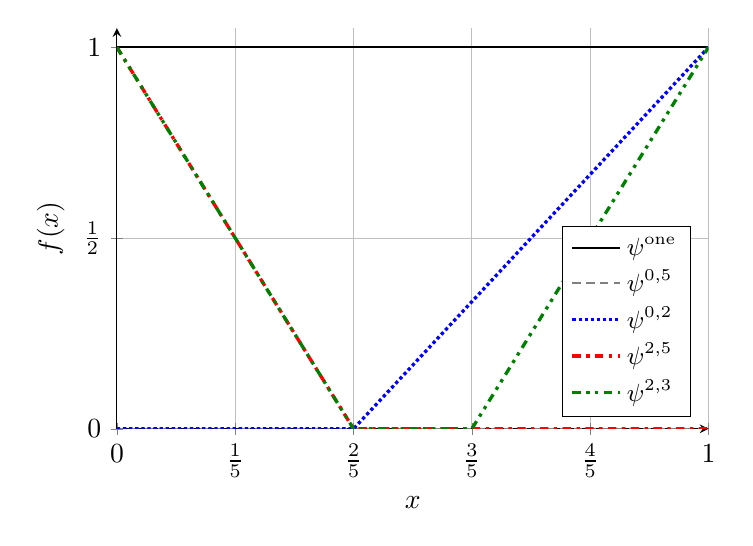
\begin{tikzpicture}
        \begin{axis}[
                width=0.75\textwidth,
                height=0.55\textwidth,
                xmin=0, xmax=1,
                ymin=0, ymax=1.05,
                axis lines=left,
                grid=both,
                xtick={0,0.2,0.4,0.6,0.8,1.0},
                xticklabels={$0$,$\tfrac{1}{5}$,$\tfrac{2}{5}$,$\tfrac{3}{5}$,$\tfrac{4}{5}$,$1$},
                ytick={0,0.5,1.0},
                yticklabels={$0$,$\tfrac{1}{2}$,$1$},
                xlabel={$x$},
                ylabel={$f(x)$},
                legend style={legend pos=south east, font=\small},
                legend cell align=left
            ]

            % constant 1: psi^{one} -- solid black
            \addplot[thick, black, solid]
            coordinates {
                    (0,1) (0.2,1) (0.4,1) (0.6,1) (0.8,1) (1,1)
                };
            \addlegendentry{$\psi^{\mathrm{one}}$}

            % constant 0: psi^{0,5} -- gray, densely dashed
            \addplot[thick, gray, densely dashed]
            coordinates {
                    (0,0) (0.2,0) (0.4,0) (0.6,0) (0.8,0) (1,0)
                };
            \addlegendentry{$\psi^{0,5}$}

            % left ramp: psi^{0,2} -- blue, densely dotted
            \addplot[very thick, blue, densely dotted]
            coordinates {
                    (0,0)
                    (0.2,0)
                    (0.4,0)
                    (0.6,1/3)
                    (0.8,2/3)
                    (1,1)
                };
            \addlegendentry{$\psi^{0,2}$}

            % right ramp: psi^{2,5} -- red, dash-dotted
            \addplot[very thick, red, dashdotted]
            coordinates {
                    (0,1)
                    (0.2,1/2)
                    (0.4,0)
                    (0.6,0)
                    (0.8,0)
                    (1,0)
                };
            \addlegendentry{$\psi^{2,5}$}

            % valley: psi^{2,3} -- greenish, dash dot dot
            \addplot[very thick, green!50!black, dash dot dot]
            coordinates {
                    (0,1)
                    (0.2,1/2)
                    (0.4,0)
                    (0.6,0)
                    (0.8,1/2)
                    (1,1)
                };
            \addlegendentry{$\psi^{2,3}$}

        \end{axis}
    \end{tikzpicture}
    \caption{Examples of one-dimensional convex basis functions on a grid of
        $m=6$ points $z_i = i/5$. Each curve corresponds to an extreme point of
        the discrete convexity polytope $\cC_m$.}
    \label{fig:convex-basis-1d}
\end{figure}

\subsubsection{Basis functions of 1d convex functions}
Recall the grid $Z=\{z_0,\dots,z_{m-1}\}$ with $z_i = i/(m-1)$ and the identification
of a convex function $f:[0,1]\to[0,1]$ with the vector
$v=(v_0,\dots,v_{m-1})\in[0,1]^m$ given by $v_i=f(z_i)$.
Discrete convexity on $Z$ is equivalent to the second–difference inequalities
\[
    v_{i-1} - 2v_i + v_{i+1} \;\ge\; 0,
    \qquad i=1,\dots,m-2.
\]
Let
\[
    \cC_m
    \;=\;
    \bigl\{
    v\in[0,1]^m:
    v_{i-1}-2v_i+v_{i+1}\ge 0 \text{ for all } i=1,\dots,m-2
    \bigr\}
\]
be the corresponding convex polytope of discretized convex functions.

\begin{definition}[Canonical convex basis vectors]
    For integers $0\le a\le b\le m-1$, define $\psi^{a,b}\in[0,1]^m$ by
    \begin{equation*}
        \psi^{a,b}_i
        \;=\;
        \begin{cases}
            1 - \dfrac{i}{a},       & 0\le i\le a,\ \ a>0,     \\[6pt]
            0,                      & a\le i\le b,             \\[6pt]
            \dfrac{i-b}{\,m-1-b\,}, & b\le i\le m-1,\ \ b<m-1,
        \end{cases}
    \end{equation*}
    with the obvious conventions that the first branch is omitted when $a=0$, the
    third branch is omitted when $b=m-1$, and when $(a,b)=(0,m-1)$ we get
    $\psi^{0,m-1}\equiv 0$.

    In other words, the function represented by $\psi^{a,b}$:
    \begin{itemize}
        \item is equal to $0$ on all grid points $z_i$ with $a\le i\le b$;
        \item is linear on $\{z_0,\dots,z_a\}$ and (if $a>0$) satisfies
              $\psi^{a,b}_0=1$, $\psi^{a,b}_a=0$;
        \item is linear on $\{z_b,\dots,z_{m-1}\}$ and (if $b<m-1$) satisfies
              $\psi^{a,b}_b=0$, $\psi^{a,b}_{m-1}=1$.
    \end{itemize}
    We also define the all–ones vector
    \[
        \psi^{\mathrm{one}} \;=\; (1,\dots,1) \in [0,1]^m.
    \]
    Finally, let
    \[
        \cB_m
        \;:=\;
        \{\psi^{\mathrm{one}}\}
        \;\cup\;
        \{\psi^{a,b}: 0\le a\le b\le m-1\}.
    \]
\end{definition}

\begin{theorem}[Extreme points of \texorpdfstring{$\cC_m$}{C\_m}]\label{thm:1d-basis}
    Every element of $\cB_m$ lies in $\cC_m$, and $\cB_m$ is exactly the set of
    extreme points of $\cC_m$.
    Consequently,
    \[
        \cC_m \;=\; \conv(\cB_m),
    \]
    so $\cB_m$ is a convex basis of discretized convex functions on $Z$.
    In particular, the number of basis vectors is
    \[
        d \;=\; |\cB_m|
        \;=\;
        1 + \Bigl|\{(a,b):0\le a\le b\le m-1\}\Bigr|
        \;=\;
        1 + \frac{m(m+1)}{2}
        \;=\;
        \frac{m^2+m+2}{2}.
    \]
    Thus one can take $\{\phi_1,\dots,\phi_d\}$ in the discussion above to be any
    enumeration of $\cB_m$.
\end{theorem}
\noindent The proof is deferred to \ref{proof:thm:1d-basis}.




\subsubsection{A sanity check---$d$-armed adversarial bandit and \expthree}
\expthree is a classical algorithm for the $d$-armed adversarial bandit problem.
This algorithm is of special interest to us since it uses affine estimators
\begin{align*}
    E(x,y) & = \frac{y}{p_x} e_x\,,
\end{align*}
where $p_x$ is the probability of choosing action $x$.
Written differently, \expthree uses an affine estimator (as defined above)
with $T_1(x) = \frac{1}{p_x} e_x$ and $T_0(x) = 0$.
This shows that \expthree fits into our setup.

\textit{Technically speaking}, there are two different versions of the
$d$-armed adversarial bandit problem: (1) the action set is the simplex
$\Delta(d)$, and (2) the action set is the set of standard basis vectors
$\{e_1, \ldots, e_d\}$.
To make the distinction clear,
suppose it's round $t$ and the loss vector is $\ell_t \in [0,1]^d$.
We have four possible scenarios:
\begin{center}
    \begin{tabular}{|c|p{5.5cm}|p{5.5cm}|}
        \hline
                           & \textbf{Action set $\Delta(d)$}                                                                                                                         & \textbf{Action set $\{e_1, \ldots, e_d\}$}                                                                                                                     \\
        \hline
        \textbf{Full-inf.} & \textbf{Plays:} $a_t \in \Delta(d)$ \newline \textbf{Observes:} $\ell_t$ \newline \textbf{Suffers:} $\langle a_t, \ell_t \rangle$
                           & \textbf{Plays:} $I_t \sim a_t$ \newline \textbf{Observes:} $\ell_t$ \newline \textbf{Suffers:} $\ell_{t, I_t}$ (expected $\langle a_t, \ell_t \rangle$)                                                                                                                                                                  \\
        \hline
        \textbf{Bandit}    & \textbf{Plays:} $a_t \in \Delta(d)$ \newline \textbf{Observes:} $\langle a_t, \ell_t \rangle$ \newline \textbf{Suffers:} $\langle a_t, \ell_t \rangle$  & \textbf{Plays:} $I_t \sim a_t$ \newline \textbf{Observes:} $\ell_{t, I_t}$ \newline \textbf{Suffers:} $\ell_{t, I_t}$ (expected $\langle a_t, \ell_t \rangle$) \\
        \hline
    \end{tabular}
\end{center}


In this subsection we instantiate the \expbyopt\ setup with the classical
\expthree\ choices on the $d$-armed simplex and obtain a uniform
(per-round, worst-case) bound on $\Lambda$. Plugging this bound into
Theorem~\ref{thm:SMD-biased} recovers the usual
$\cO\!\left(\sqrt{dn\ln d}\right)$ regret.
\begin{proposition}[Per-round $\Lambda$ bound for \expthree]\label{prop:Lambda-Exp3}
    Let $\cA=\{e_1,\ldots,e_d\}$ and $F=R$ be the negentropy on $\Delta(d)$.
    Fix a round with MD iterate $a\in\Delta(d)$ and learning rate $\eta>0$.
    Let the exploration distribution be $P$ with
    $\P(A=e_i)=a_i$ (so $\E[A]=a$), and use the standard loss-based
    importance-weighted estimator
    \(
    \hl \equiv E(A,Y)=\frac{Y}{a_I}e_I
    \)
    with $I\sim a$ and $Y=\ip{A,\ell}=\ell_I$ for a loss vector $\ell\in[0,1]^d$.
    Then for every comparator $a_\star\in\Delta(d)$,
    \begin{align}
        \Lambda_{a,\eta}(P,E\!\mid\mid a_\star,\ell)
         & =
        \frac{1}{\eta^2}\,
        \E\!\Big[D_{R^\star}\big(R'(a)-\eta \hl,R'(a)\big)\Big]
        \;\le\;
        \frac{1}{2}\,\|\ell\|_2^2
        \;\le\;
        \frac{d}{2}\,.
        \label{eq:Lambda-Exp3-bound}
    \end{align}
    The inequality is uniform in $a\in\Delta(d)$ and $\eta>0$.
\end{proposition}
The proof is deferred to \ref{proof:prop:Lambda-Exp3}.
\subsubsection{The optimal affine estimator}


\clearpage
\bibliographystyle{plainnat}
\bibliography{all}
\clearpage

\appendix
\section{Appendix}
\label{sec:appendix}
\subsection{Proofs of \expbyopt}
\begin{lemma}[Alternative $\Lambda(P, E || \nu)$]
    We have
    \begin{align}
        \Lambda(P, E || \nu)
        =
        \frac{1}{\eta}
        \left(
        \Delta(\nu, P) +
        \E\!\left[
                \langle A_\star, \hl \rangle
                + \frac{1}{\eta} F^\star\left(F'(a) - \eta \hl\right)
                - \frac{1}{\eta} F^\star(F'(a))
                \right]
        \right)
        \,.
        \label{eq:Lambda-simplified}
    \end{align}
\end{lemma}
\begin{proof}
    With $\hl = E(A, Y)= E(A, \langle A, \ell \rangle)$, we have
    \begin{align}
        \eta \Lambda(P, E || \nu)
         & =
        \E\!\left[
            \langle A - A_\star, \ell \rangle
            - \langle a - A_\star, \hl \rangle
            + \frac{1}{\eta} D_{F^\star}(F'(a) - \eta \hl, F'(a))
            \right]
        \nonumber \\
         & =
        \Delta(\nu, P) +
        \E\!\left[
        \langle A_\star - a, \hl \rangle
        + \frac{1}{\eta}
        \left(
        F^\star\left(F'(a) - \eta \hl\right)
        - F^\star(F'(a))
        - {F^\star}'(F'(a))^\top (- \eta \hl)
        \right)
        \right]
        \nonumber \\
         & =
        \Delta(\nu, P) +
        \E\!\left[
            \langle A_\star - a, \hl \rangle
            + \frac{1}{\eta}
            \left(
            F^\star\left(F'(a) - \eta \hl\right)
            - F^\star(F'(a))
            + \eta a^\top \hl
            \right)
            \right]
        \nonumber \\
         & =
        \Delta(\nu, P) +
        \E\!\left[
            \langle A_\star, \hl \rangle
            + \frac{1}{\eta} F^\star\left(F'(a) - \eta \hl\right)
            - \frac{1}{\eta} F^\star(F'(a))
            \right]\,.
        \nonumber
    \end{align}
\end{proof}
\subsubsection{Proof of lemma~\ref{lem:optimal-E}}
\label{proof:lem:optimal-E}
\begin{proof}[Proof of lemma~\ref{lem:optimal-E}]
    By taking the derivative of $\Lambda(P, E || \nu)$ with respect to $E(b,y)$
    for any pair $(b,y) \in \cA \times \R$ we have
    \begin{align*}
        \tfrac{\partial}{\partial E(b,y)} \Lambda_\eta(P, E || \nu)
         & =
        \tfrac{\partial}{\partial E(b,y)}
        \left(
        \frac{1}{\eta}
        \left(
            \Delta(\nu, P) +
            \E\!\left[
                    \langle A_\star, \hl \rangle
                    + \frac{1}{\eta} F^\star\left(F'(a) - \eta \hl\right)
                    - \frac{1}{\eta} F^\star(F'(a))
                    \right]
            \right)
        \right)
        \\
         & =
        \tfrac{\partial}{\partial E(b,y)}
        \left(
        \frac{1}{\eta}
        \E\!\left[
                \langle A_\star, \hl \rangle
                + \frac{1}{\eta} F^\star\left(F'(a) - \eta \hl\right)
                \right]
        \right) \\
         & =
        \tfrac{\partial}{\partial E(b,y)}
        \tfrac{\P(A=b, Y=y)}{\eta}
        \E\!\left[
            \langle A_\star, \hl \rangle
            + \frac{1}{\eta} F^\star\left(F'(a) - \eta \hl\right)
            \bigg| A = b, Y = y
        \right] \\
         & =
        \tfrac{\partial}{\partial E(b,y)}
        \tfrac{\P(A=b, Y=y)}{\eta}
        \E\!\left[
            \langle A_\star, E(b, y) \rangle
            + \frac{1}{\eta} F^\star\left(F'(a) - \eta E(b, y)\right)
            \bigg|A = b, Y = y
        \right] \\
         & =
        \tfrac{\P(A=b, Y=y)}{\eta}
        \E\!\left[
        A_\star
        - {F^\star}'\left(F'(a) - \eta E(b, y)\right)
        \bigg| A = b, Y = y
        \right] \\
         & =
        \tfrac{\P(A=b, Y=y)}{\eta}
        \left(
        \E\!\left[
            A_\star
            |A = b, Y = y\right]
        - {F^\star}'\left(F'(a) - \eta E(b, y)\right)
        \right)\,,
    \end{align*}
    and by setting the gradient to zero, we get
    \begin{align*}
        \E\!\left[
            A_\star
            | A = b, Y = y\right]
         & = {F^\star}'\left(F'(a) - \eta E(b, y)\right) \\
        \Rightarrow
        F'\left(\E\!\left[
            A_\star
            | A = b, Y = y\right]\right)
         & = F'(a) - \eta E(b, y)                        \\
        \Rightarrow
        E(b, y)
         & =
        \frac{1}{\eta}
        \left(
        F'(a)
        -
        F'\left(\E\!\left[
            A_\star
            | A = b, Y = y\right]\right)
        \right)\,. \qedhere
    \end{align*}
\end{proof}

\subsubsection{Proof of lemma~\ref{lem:optimal-Lambda-wrong-turn}}
\label{proof:lem:optimal-Lambda-wrong-turn}
\begin{proof}[Proof of lemma~\ref{lem:optimal-Lambda-wrong-turn}]
    From lemma~\ref{lem:optimal-E}, the optimal estimator is
    $
        G^\nu(b, y)  =
        \frac{1}{\eta}\left(
        F'(a) - F'(\E[A_\star|\langle \ell, b\rangle = y])
        \right)$.
    By plugging in $G^\nu$ into eq~\ref{eq:Lambda-simplified}, we have
    \begin{align*}
         & \eta \Lambda(P, G^\nu|| \nu)  - \Delta(\nu, P)
        \\
         & =
        \E\!\left[
            \langle A_\star, \hl \rangle
            + \frac{1}{\eta} F^\star\left(F'(a) - \eta \hl\right)
            - \frac{1}{\eta} F^\star(F'(a))
            \right]
        \\
         & =
        \E\!\left[
            \langle A_\star, G^\nu(A, Y) \rangle
            + \frac{1}{\eta} F^\star\left(F'(a) - \eta G^\nu(A, Y)\right)
            - \frac{1}{\eta} F^\star(F'(a))
            \right]
        \\
         & =
        \E\!\left[
            \eta^{-1}\langle A_\star,
            F'(a) - F'(\E[A_\star|\langle \ell, A\rangle = Y])
            \rangle
            + \frac{1}{\eta} F^\star\left(
            F'(\E[A_\star|\langle \ell, A\rangle = Y])
            \right)
            - \frac{1}{\eta} F^\star(F'(a))
            \right]
        \\
         & =\eta^{-1}
        \E\!\bigg[
            \big\langle
            \E[A_\star|\langle \ell, A\rangle = Y],
            F'(a) - F'(\E[A_\star|\langle \ell, A\rangle = Y])
            \big\rangle
            + F^\star\left(
            F'(\E[A_\star|\langle \ell, A\rangle = Y])
            \right)
            - F^\star(F'(a))
            \bigg]
        \\
         & =
        -\eta^{-1}
        \E\!\bigg[
            D_{F^\star}\left(F'(a), F'(\E[A_\star|\langle \ell, A\rangle = Y])\right)
            \bigg]
        \\
         & =
        -\eta^{-1}
        \E\!\bigg[
            D_F\left(
            \E[A_\star|\langle \ell, A\rangle = Y], a
            \right)
            \bigg]\,. \qedhere
    \end{align*}
\end{proof}

\subsubsection{Proof of theorem~\ref{thm:optimal-Lambda-info-ratio}}
\label{proof:thm:optimal-Lambda-info-ratio}
\begin{proof}[Proof of theorem~\ref{thm:optimal-Lambda-info-ratio}]
    From lemma~\ref{lem:optimal-Lambda-wrong-turn} and lemma~\ref{lem:the-right-turn}, we have
    \begin{align*}
        \Lambda(P, G^\nu|| \nu)
         & = \frac{1}{\eta} \Delta(\nu, P)
        - \frac{1}{\eta^2}
        \E\!\left[
            D_F\left(\po, a\right)
        \right]                            \\
         & = \frac{1}{\eta} \Delta(\nu, P)
        - \frac{1}{\eta^2}
        \left(
        \E\left[
                D_F\left( \po, \pr\right)
                \right]
        +
        D_F\left( \pr, a\right)
        \right)                            \\
         & \leq \frac{
            \Delta(\nu, P)^2
        }{
            4 \E\left[D_F\left( \po, \pr\right)\right]
        }\,,
    \end{align*}
    where the first inequality is by dropping the non-negative term $D_F( \pr, a)$,
    and the second inequality is by maximizing over $\eta$.
\end{proof}

\subsubsection{Proof of theorem~\ref{thm:optimal-affine-y}}
\label{proof:thm:optimal-affine-y}
\begin{proof}[Proof of Thm~\ref{thm:optimal-affine-y}]
    Starting from eq~\ref{eq:Lambda-simplified}, we are interested in the $T$ that minimizes
    \begin{align*}
        \eta \Lambda(P, T || \nu)
         & =
        \Delta(\nu, P) +
        \E\!\left[
            \langle A_\star, \hl \rangle
            + \frac{1}{\eta} F^\star\left(F'(a) - \eta \hl\right)
            - \frac{1}{\eta} F^\star(F'(a))
            \right]\,,
    \end{align*}
    but note that the first term $\Delta(\nu, P)$
    and the last term $F^\star(F'(a))$ can be dropped
    from the optimization since they don't depend on the estimator choice
    $T$ (no $\hl$ present).

    For $x \in \cA$, we solve for $T_1^\nu(x), T_0^\nu(x)$ through differentiation.
    First, for $T_0(x)$, we have
    \begin{align*}
         & \tfrac{\partial}{\partial T_0(x)} \Lambda(P, T||\nu)
        \\
         & =
        \tfrac{\partial}{\partial T_0(x)}
        \eta^{-1}
        \E\!\left[
            \langle A_\star, \hl \rangle
            + \frac{1}{\eta} F^\star\left(F'(a) - \eta \hl\right)
            \right]
        \\
         & =
        \tfrac{P(x)}{\eta} \cdot
        \tfrac{\partial}{\partial T_0(x)}
        \E\!\left[
            \langle A_\star, Y T_1(x) + T_0(x) \rangle
            + \frac{1}{\eta} F^\star\left(F'(a) - \eta (Y T_1(x) + T_0(x))\right)
            | A = x
            \right]
        \\
         & =
        \tfrac{P(x)}{\eta} \cdot
        \tfrac{\partial}{\partial T_0(x)}
        \E\!\left[
            \langle A_\star, T_0(x) \rangle
            + \frac{1}{\eta} F^\star\left(F'(a) - \eta (Y T_1(x) + T_0(x))\right)
            | A = x
            \right]
        \\
         & =
        \tfrac{P(x)}{\eta} \cdot
        \E\!\left[
        A_\star
        - {F^\star}'\left(F'(a) - \eta (Y T_1(x) + T_0(x))\right)
        | A = x
        \right]\,,
    \end{align*}
    which by setting the derivative to zero gives
    \begin{align}
        \E\!\left[
            A_\star
            | A = x
            \right]
         & =
        \E\!\left[
            {F^\star}'\left(F'(a) - \eta \hl \right)
            | A = x
            \right]\,,
        \label{eq:t0-optimal}
    \end{align}
    for all $x \in \cA$.
    Secondly, for $T_1(x)$, we have
    \begin{align*}
         & \tfrac{\partial}{\partial T_1(x)} \Lambda(P, T||\nu)
        \\
         & =
        \tfrac{\partial}{\partial T_1(x)}
        \eta^{-1}
        \E\!\left[
            \langle A_\star, \hl \rangle
            + \frac{1}{\eta} F^\star\left(F'(a) - \eta \hl\right)
            \right]
        \\
         & =
        \tfrac{P(x)}{\eta} \cdot
        \tfrac{\partial}{\partial T_1(x)}
        \E\!\left[
            \langle A_\star, Y T_1(x) + T_0(x) \rangle
            + \frac{1}{\eta} F^\star\left(F'(a) - \eta (Y T_1(x) + T_0(x))\right)
            | A = x
            \right]
        \\
         & =
        \tfrac{P(x)}{\eta} \cdot
        \tfrac{\partial}{\partial T_1(x)}
        \E\!\left[
            \langle A_\star, Y T_1(x) \rangle
            + \frac{1}{\eta} F^\star\left(F'(a) - \eta (Y T_1(x) + T_0(x))\right)
            | A = x
            \right]
        \\
         & =
        \tfrac{P(x)}{\eta} \cdot
        \E\!\left[
            Y A_\star
            - Y {F^\star}'\left(F'(a) - \eta (Y T_1(x) + T_0(x))\right)
            | A = x
            \right]\,,
    \end{align*}
    and by setting the derivative to zero, we have
    \begin{align}
        \E\!\left[
            Y A_\star
            | A = x
            \right]
         & =
        \E\!\left[
            Y {F^\star}'\left(F'(a) - \eta \hl \right)
            | A = x
            \right]
        \label{eq:t1-optimal}
    \end{align}
    for all $x \in \cA$.
    Finally, combining eqs~\ref{eq:t0-optimal} and~\ref{eq:t1-optimal}
    we have
    \begin{align*}
        \E\left[
            \hl A_\star|A=x
            \right]
         & =
        \E\left[
            (T_1(x) Y + T_0(x)) A_\star|A=x
        \right] \\
         & =
        T_1(x)
        \E\left[
            Y A_\star|A=x
            \right]
        + T_0(x)
        \E\left[
            A_\star|A=x
        \right] \\
         & =
        T_1(x)
        \E\left[
            Y {F^\star}'\left(F'(a) - \eta \hl \right)
            | A = x
            \right]
        +
        T_0(x)
        \E\left[
            {F^\star}'\left(F'(a) - \eta \hl \right)
            | A = x
        \right] \\
         & =
        \E\left[
            \hl
            {F^\star}'\left(F'(a) - \eta \hl \right)
            | A = x
            \right]\,,
    \end{align*}
    which concludes the proof.
\end{proof}

\subsubsection{Proof of lemma~\ref{lem:E-optimized-Lambda}}
\label{proof:lem:E-optimized-Lambda}
\begin{proof}[Proof of lemma~\ref{lem:E-optimized-Lambda}]
    Starting from eq~\ref{eq:Lambda-simplified}, we have
    \begin{align*}
        \eta \Lambda(P, E_{T^\nu} || \nu)
         & =
        \Delta(\nu, P) +
        \E\!\left[
            \langle A_\star, \hl \rangle
            + \frac{1}{\eta} F^\star\left(F'(a) - \eta \hl\right)
            - \frac{1}{\eta} F^\star(F'(a))
            \right]
        \\
         & =
        \Delta(\nu, P) +
        \E\!\left[
            \E\!\left[
                \langle A_\star, \hl \rangle
                + \frac{1}{\eta} F^\star\left(F'(a) - \eta \hl\right)
                - \frac{1}{\eta} F^\star(F'(a))
                \bigg|
                A
                \right]
            \right]
        \\
         &
        \abovelabel{by eq~\ref{eq:affine-E-opt}}
        =
        \Delta(\nu, P) +
        \E\!\left[
            \E\!\left[
                \langle {F^\star}'\left(F'(a) - \eta \hl\right), \hl \rangle
                + \frac{1}{\eta} F^\star\left(F'(a) - \eta \hl\right)
                - \frac{1}{\eta} F^\star(F'(a))
                \bigg|
                A
                \right]
            \right]
        \\
         & =
        \Delta(\nu, P) -
        \frac{1}{\eta}
        \E\!\left[
            D_{F^\star}\left(F'(a), F'(a) - \eta \hl\right)
            \right]\,.
    \end{align*}
\end{proof}

\subsubsection{Proof of theorem~\ref{thm:affine-Y-Lambda-info-ratio}}
\label{proof:thm:affine-Y-Lambda-info-ratio}
\begin{proof}[Proof of theorem~\ref{thm:affine-Y-Lambda-info-ratio}]
    Start from the optimality condition for affine-$Y$ estimators,
    we have
    \begin{equation}
        \E\!\left[\hl \odot A_\star \,\middle|\, A \right]
        \;=\;
        \E\!\left[\hl \odot \tilde{A} \,\middle|\, A \right]
        \quad \Rightarrow \quad
        \E\!\left[\hl \odot \left(A_\star-\tilde{A}\right) \,\middle|\, A \right] \;=\; 0
        \,.
        \tag{\ref{eq:affine-E-opt}}
    \end{equation}
    Next, by tower rule and conditioning further on $(A,Y)$ we get
    \begin{align}
        0 & = \E\!\left[\hl \odot \left(A_\star-\tilde{A}\right) \,\middle|\, A \right] \nonumber \\
          & = \E\!\left[
            \E\!\left[\hl \odot \left(A_\star-\tilde{A}\right) \,\middle|\, A, Y \right]
            \,\middle|\, A
        \right]                                                                         \nonumber \\
          & = \E\!\left[
            \hl \odot
            \left(\po-\tilde{A}\right)
            \,\middle|\, A
            \right]\,,
        \label{eq:tildeA-vs-po}
    \end{align}
    where in the last step we used that $\tilde{A}$ and $\hl$ are functions of $(A,Y)$
    and that $\po=\E[A_\star|A,Y]$.
    % hence
    % \begin{equation}
    %     \E\!\left[\hl \odot \left(\po - \tilde{A}\right) \,\middle|\, A \right] \;=\; 0.
    %     \label{eq:tildeA-vs-po}
    % \end{equation}
    Next, use the defining relation
    \begin{equation}
        F'(a) - F'(\tilde{A}) \;=\; \eta\,\hl,
        \tag{\ref{eq:hl-alternate}}
    \end{equation}
    together with \eqref{eq:tildeA-vs-po} gives
    \[
        \E\!\left[
            \left\langle F'(a) - F'(\tilde{A}),\, \po - \tilde{A} \right\rangle
            \,\middle|\, A
            \right] \;=\; 0.
    \]
    Taking total expectation and applying the Bregman three‑point identity
    \(
    \langle F'(z)-F'(y),\,x-y\rangle
    = D_F(x,y)+D_F(y,z)-D_F(x,z)
    \)
    with $(x,y,z)=(\po,\tilde{A},a)$ yields
    \[
        \E\!\left[D_F(\po,\tilde{A}) + D_F(\tilde{A}, a)\right]
        \;=\;
        \E\!\left[D_F(\po, a)\right].
    \]
    By the expected Bregman identity (Lemma~\ref{lem:the-right-turn}),
    \(
    \E[D_F(\po, a)] = \E[D_F(\po,\pr)] + D_F(\pr,a).
    \)
    Therefore,
    \begin{equation}
        \E\!\left[D_F(\po,\tilde{A})\right] + \E\!\left[D_F(\tilde{A}, a)\right]
        \;=\;
        \E\!\left[D_F(\po,\pr)\right] + D_F(\pr,a).
        \label{eq:EBI-key}
    \end{equation}

    Now apply the assumption with $a=\pr$:
    \(
    \E[D_F(\tilde{A}, \pr)] \ge \E[D_F(\po,\pr)].
    \)
    Plugging this into \eqref{eq:EBI-key} with $a=\pr$ gives
    \[
        \E\!\left[D_F(\po,\tilde{A})\right] + \underbrace{\E\!\left[D_F(\tilde{A}, \pr)\right]}_{\ge \,\E[D_F(\po,\pr)]}
        \;\le\;
        \E\!\left[D_F(\po,\pr)\right],
    \]
    hence $\E[D_F(\po,\tilde{A})] \le 0$. Since Bregman divergences are non‑negative and vanish iff their arguments coincide (for strictly convex differentiable $F$), we conclude $D_F(\po,\tilde{A})=0$ almost surely, i.e., $\tilde{A}=\po$ a.s.
\end{proof}

\subsubsection{Proof of theorem~\ref{thm:no-alpha}}
\label{proof:thm:no-alpha}
\begin{proof}[Proof of Thm.~\ref{thm:no-alpha}]
    Let $Z\sim\cN(0,1)$ and fix parameters $\beta,\omega>0$. Define
    \[
        A_\star = \big(-\beta Z,\;\omega(Z^2-1),\;0,\cdots,0\big),\qquad
        \ell = (Z,0,\cdots,0).
    \]
    Take the sampling rule $P$ that plays deterministically $A=e_1$, so
    $Y=\langle \ell, A\rangle = Z$. The prior mean is $\pr=\E[A_\star]=0$ and,
    since $A_\star$ is a deterministic function of $Y$, the posterior mean is
    \(
    \po=\E[A_\star\mid A,Y]=A_\star.
    \)

    Let $T$ be any optimizer in the affine-$Y$ class guaranteed by
    Thm.~\ref{thm:optimal-affine-y}, which satisfies the first‑order condition
    \eqref{eq:affine-E-opt}:
    \[
        \E\!\left[\hl\odot A_\star \,\middle|\, A\right]
        \;=\;
        \E\!\left[\hl\odot \tilde{A} \,\middle|\, A\right],
        \qquad \text{where }\;\hl=Y\,T_A,\;\;
        \tilde{A}={F^\star}'\!\left(F'(a)-\eta\hl\right).
    \]
    For the quadratic potential, $F'(x)=x$ and ${F^\star}'(q)=q$, hence
    $\tilde{A}=a-\eta\hl$. Taking $a=\pr=0$ yields $\tilde{A}=-\eta\hl=-\eta Y T_A$.

    Conditioning on $A=e_1$ and using $Y=Z$, the optimality condition becomes
    \[
        \E\!\left[\, Z\,T_{e_1}\odot A_\star\,\right]
        \;=\;
        \E\!\left[\, Z\,T_{e_1}\odot(-\eta Z T_{e_1})\,\right]
        \;=\;
        -\eta\,\E[Z^2]\,(T_{e_1}\odot T_{e_1})
        \;=\;
        -\eta\,(T_{e_1}\odot T_{e_1}).
    \]
    Since $\E[Z^2]=1$ and $\E[Z(Z^2-1)]=0$, the left side equals
    $(-\beta T_{e_1,1},0,\cdots,0)$. Therefore
    \[
        -\beta T_{e_1,1}=-\eta T_{e_1,1}^2,\qquad
        -\eta T_{e_1,j}^2=0\ (j\ge 2),
    \]
    which forces $T_{e_1,1}=\beta/\eta$ and $T_{e_1,j}=0$ for $j\ge 2$. Consequently,
    \[
        \tilde{A}=-\eta Y T_{e_1}=-\beta Z\,e_1.
    \]

    Now compute the two divergences (for $F(x)=\tfrac12\|x\|^2$, $D_F(u,0)=\tfrac12\|u\|^2$):
    \[
        \E\!\left[D_F(\tilde{A},\pr)\right]
        =\tfrac12\,\E\!\left[\|\tilde{A}\|^2\right]
        =\tfrac12\,\beta^2,
        \quad
        \E\!\left[D_F(\po,\pr)\right]
        =\tfrac12\,\E\!\left[\|A_\star\|^2\right]
        =\tfrac12\big(\beta^2+2\omega^2\big),
    \]
    using $\E[Z^2]=1$ and $\E[(Z^2-1)^2]=2$. Hence
    \[
        \frac{\E[D_F(\tilde{A},\pr)]}{\E[D_F(\po,\pr)]}
        =\frac{\beta^2}{\beta^2+2\omega^2}.
    \]
    Letting $\omega\to\infty$ drives the ratio to $0$, which shows that no uniform
    $\alpha>0$ can lower‑bound this ratio across priors and sampling rules.
\end{proof}

% \subsubsection{Proof of proposition~\ref{prop:Lambda-Exp3}}
\label{proof:prop:Lambda-Exp3}
\begin{proof}[Proof of proposition~\ref{prop:Lambda-Exp3}]
    By unbiasedness, $\E[\hl]=\ell$, and by construction $\E[A]=a$. Hence the
    linear terms in the definition of $\Lambda$ cancel in expectation:
    \begin{align*}
        \Lambda_{a,\eta}(P,E\!\mid\mid a_\star,\ell)
         & =\frac{1}{\eta}\,\E\!\Big[\ip{A-a_\star,\ell}-\ip{a-a_\star,\hl}
        +\frac{1}{\eta}D_{F^\star}(F'(a)-\eta \hl,F'(a))\Big]                  \\
         & =\frac{1}{\eta^2}\,\E\!\big[D_{F^\star}(F'(a)-\eta \hl,F'(a))\big].
    \end{align*}
    For negentropy $F=R$, we have $R'(a)=\ln a$ (componentwise),
    $R^\star(q)=\sum_i e^{q_i}$, and, for any $z\in\R^d$,
    \begin{align*}
        D_{R^\star}(\ln a-\eta z,\ln a)
         & = R^\star(\ln a-\eta z)-R^\star(\ln a)
        - R'^\star(\ln a)^\top(-\eta z)                         \\
         & =\sum_{i=1}^d a_i\Big(e^{-\eta z_i}-1+\eta z_i\Big).
    \end{align*}
    Taking $z=\hl$ and recalling that under the estimator
    $\hl_I=\ell_I/a_I$ and $\hl_i=0$ for $i\neq I$, we obtain
    \[
        D_{R^\star}(\ln a-\eta \hl,\ln a)
        = a_I\!\left(e^{-\eta \ell_I/a_I}-1\right)+\eta \ell_I.
    \]
    Averaging over $I\sim a$ yields
    \begin{align}
        \E\!\big[D_{R^\star}(\ln a-\eta \hl,\ln a)\big]
         & =\sum_{i=1}^d a_i^2\!\left(e^{-\eta \ell_i/a_i}-1\right)+\eta \sum_{i=1}^d a_i \ell_i.
        \label{eq:exact-exp3-D}
    \end{align}
    Using the elementary bound $e^{-x}\le 1-x+\tfrac{x^2}{2}$ for all $x\ge 0$
    (with $x=\eta \ell_i/a_i$; note $\ell_i\ge 0$ and $a_i>0$), we get
    \[
        a_i^2\!\left(e^{-\eta \ell_i/a_i}-1\right)
        \le -\eta a_i\ell_i+\frac{\eta^2}{2}\,\ell_i^2.
    \]
    Summing this over $i$ and adding the $+\eta\sum_i a_i\ell_i$ term in
    \eqref{eq:exact-exp3-D} produces a cancellation, giving
    \[
        \E\!\big[D_{R^\star}(\ln a-\eta \hl,\ln a)\big]
        \le \frac{\eta^2}{2}\sum_{i=1}^d \ell_i^2
        = \frac{\eta^2}{2}\,\|\ell\|_2^2.
    \]
    Dividing by $\eta^2$ proves the first inequality in
    \eqref{eq:Lambda-Exp3-bound}. Since $\ell\in[0,1]^d$,
    $\|\ell\|_2^2\le d$, which yields the second inequality.
\end{proof}
\subsubsection{Proof of theorem~\ref{thm:fixed-action-per-loss}}
\label{proof:thm:fixed-action-per-loss}
\begin{proof}[Proof of theorem~\ref{thm:fixed-action-per-loss}]
    Observe that
    \begin{align*}
        \po & = \E[A_\star|A, Y] \\
            & = \E\left[
            \E[A_\star|\ell, A, Y]
            | A, Y
        \right]                  \\
            & = \E\left[
            \E[A_\star|\ell, A]
            | A, Y
            \right]
        \tag{$Y = \langle A, \ell \rangle$}
        \\
            & = \E\left[
            \E[A_\star|\ell]
            | A, Y
            \right]\,,
        \tag{$A_\star$ is independent of $A$ given $\ell$}
    \end{align*}
    so defining
    \begin{align*}
        a_\star(\ell) & = \E[A_\star|\ell]\,,
    \end{align*}
    we have $\po = \E\left[
            a_\star(\ell)
            | A, Y
            \right]$.
    Next, recall the value of $\Lambda(P, G^{\nu} || \nu)$ from lemma~\ref{lem:optimal-Lambda-wrong-turn}:
    \begin{align*}
        \Lambda(P, G^{\nu} || \nu)
         & = \frac{1}{\eta}
        \Delta(\nu, P)
        - \frac{1}{\eta^2}
        \E\!\left[
            D_F\left( \po, a\right)
        \right]                                      \\
         & =
        \frac{1}{\eta}
        \E\left[
            \langle A - A_\star, \ell\rangle
            \right]
        - \frac{1}{\eta^2}
        \E\!\left[
            D_F\left( \E[a_\star(\ell)|A, Y], a\right)
        \right]                                      \\
         & =
        \frac{1}{\eta}
        \E\left[
            \langle A - \E[A_\star|\ell], \ell\rangle
            \right]
        - \frac{1}{\eta^2}
        \E\!\left[
            D_F\left( \E[a_\star(\ell)|A, Y], a\right)
        \right]                                      \\
         & =
        \frac{1}{\eta}
        \E\left[
            \langle A - a_\star(\ell), \ell\rangle
            \right]
        - \frac{1}{\eta^2}
        \E\!\left[
            D_F\left( \E[a_\star(\ell)|A, Y], a\right)
        \right]                                      \\
         & = \Lambda(P, G^{\nu'} || \nu')\,.\qedhere
    \end{align*}
\end{proof}

\subsubsection{Proof of lemma~\ref{lem:mu-concave}}
\label{proof:lem:mu-concave}
\begin{proof}[Proof of lemma~\ref{lem:mu-concave}]
    By Lemma~\ref{lem:optimal-Lambda-wrong-turn}, for $\nu=\nu(\mu,a_\star)$,
    \begin{align}
        \Phi(\mu,a_\star)
         & = \frac{1}{\eta}\,\Delta(\nu,P) \;-\; \frac{1}{\eta^2}\,
        \E\!\left[D_F\!\left(\po,a\right)\right],
        \qquad \po=\E\!\left[a_\star(\ell)\,\middle|\,A,Y\right].
        \label{eq:phi-decomp}
    \end{align}
    The first term is
    \[
        \Delta(\nu,P)
        = \E\!\left[\ip{A-a_\star(\ell),\,\ell}\right]
        = \E\!\left[\ip{A,\ell}\right] - \E\!\left[\ip{a_\star(\ell),\ell}\right],
    \]
    where the first expectation is linear in $\mu$.
    The second expectation is bilinear in $(\mu,a_\star)$,
    but we need to show concavity of the entire term
    $(\mu,a_\star)\mapsto \E[D_F(\po,a)]$.
    To this end, we have
    \begin{align*}
        \E\!\left[D_F(\po,a)\right]
         & = \E\!\left[F(\po)\right] - F(a) - F'(a)^\top (\E[\po]-a) \\
         & = \E\!\left[F(\po)\right] - F'(a)^\top \E[\po] + c(a),
    \end{align*}

    For the second term, use the Bregman form
    $D_F(x,a)=F(x)-F'(a)^\top x + c(a)$,
    to write
    \[
        \E\!\left[D_F(\po,a)\right]
        = \E\!\left[F(\po)\right] - F'(a)^\top \E[\po] + c(a)
        = \E\!\left[F(\po)\right] - F'(a)^\top \E[a_\star(\ell)] + c(a),
    \]
    where we used $\E[\po]=\E[a_\star(\ell)]$.
    Thus convexity of $(\mu,a_\star)\mapsto \E[D_F(\po,a)]$ reduces to convexity of
    $(\mu,a_\star)\mapsto \E[F(\po)]$.

    By Fenchel–Young,
    $F(u)=\sup_{q\in\Rd}\{\ip{q,u}-F^\star(q)\}$.
    Applying this pointwise to $u=\po=\E[a_\star(\ell)\mid A,Y]$ and using a measurable
    selection for the maximizer (or taking the supremum over measurable $Q:\cA\times\R\to\Rd$) yields
    \begin{align*}
        \E\!\left[F(\po)\right]
         & = \sup_{Q}\,
        \left\{
        \E\!\left[\ip{Q(A,Y),\,\po}\right] - \E\!\left[F^\star(Q(A,Y))\right]
        \right\}        \\
         & = \sup_{Q}\,
        \left\{
        \E\!\left[\ip{Q(A,Y),\,a_\star(\ell)}\right] - \E\!\left[F^\star(Q(A,Y))\right]
        \right\},
    \end{align*}
    where we used the tower property
    $\E[\ip{Q(A,Y),\po}]=\E[\ip{Q(A,Y),a_\star(\ell)}]$.
    For fixed $Q$, the functional
    \(
    (\mu,a_\star)\mapsto \E[\ip{Q(A,Y),a_\star(\ell)}] - \E[F^\star(Q(A,Y))]
    \)
    is affine in $(\mu,a_\star)$ (linear in the law of $(A,Y)$—hence in $\mu$—and linear in $a_\star$).
    A supremum of affine functionals is convex. Hence
    $(\mu,a_\star)\mapsto \E[F(\po)]$ is convex, so
    $(\mu,a_\star)\mapsto \E[D_F(\po,a)]$ is convex, and by \eqref{eq:phi-decomp},
    $(\mu,a_\star)\mapsto \Phi(\mu,a_\star)$ is concave.
\end{proof}

\subsubsection{Proof of theorem~\ref{thm:binary-hypercube-losses}}
\label{proof:thm:binary-hypercube-losses}
\begin{proof}[Proof of theorem~\ref{thm:binary-hypercube-losses}]
    Recall the definitions of $\po$ and $\tilde{A}$:
    \begin{align*}
        \po       & = \E[a_\star(\ell) | A, Y]\,,          \\
        \tilde{A} & = {F^\star}'\left(F'(a) - \eta \right)
        = {F^\star}'\left(F'(a) - \eta (T_1(A)Y + T_0(A))\right)\,,
    \end{align*}
    where $a_\star$ is the function defined in theorem~\ref{thm:fixed-action-per-loss}.

    Since the action space is the $k$-simplex,
    we have $A = e_I$ for some random variable $I \in [k]$ with
    $\P(I = i) = P_i$.
    Also, since $\ell$ is supported on $\{0,1\}^k$,
    we have $Y = \langle e_I, \ell \rangle = \ell_I$.
    Therefore, we can rewrite $\po$ as
    \begin{align*}
        \po & = \E[a_\star(\ell) | I, \ell_I]\,,
    \end{align*}
    and we can rewrite $\tilde{A}$ as
    \begin{align*}
        \tilde{A} & = {F^\star}'\left(F'(a) - \eta (T_1(e_I)\ell_I + T_0(e_I))\right)\,.
    \end{align*}

    Note that $\ell_I$ is a Bernoulli random variable
    given $I$ since $\ell$ is supported on $\{0,1\}^k$.
    Therefore, for every fixed $i \in [k]$,
    we can choose $T_1(e_i)$ and $T_0(e_i)$ as
    \begin{align*}
        T_0(e_i) & = \frac{1}{\eta}
        \left(F'(a) - F'(\E[a_\star(\ell) | I = i, \ell_i = 0])\right)\,, \\
        T_1(e_i) & = \frac{1}{\eta}
        \left(F'(\E[a_\star(\ell) | I = i, \ell_i = 0])
        - F'(\E[a_\star(\ell) | I = i, \ell_i = 1])\right)\,,
    \end{align*}
    which results in
    \begin{align*}
        \tilde{A} & =
        {F^\star}'\left(F'(a) - \eta (T_1(e_I)\ell_I + T_0(e_I))\right) \\
                  & =
        \E[a_\star(\ell) | I, \ell_I] = \po\,,
    \end{align*}
    almost surely.
\end{proof}

\subsection{Proof of theorem~\ref{thm:1d-basis}}
\label{proof:thm:1d-basis}
\begin{proof}[Proof of theorem~\ref{thm:1d-basis}]
    \emph{Step 1: $\cC_m$ is the discretization of convex functions on $[0,1]$.}
    Given $v\in\cC_m$, define $f:[0,m-1]\to\R$ to be the continuous, piecewise
    affine function with $f(i)=v_i$ and affine on each $[i,i+1]$.
    The inequalities $v_{i-1}-2v_i+v_{i+1}\ge 0$ are equivalent to the slopes
    $f(i)-f(i-1)$ forming a nondecreasing sequence, hence $f$ is convex.
    Conversely, the sampled values of any convex $f$ on $\{0,\dots,m-1\}$ satisfy
    these inequalities.
    The box constraints $0\le v_i\le 1$ translate to $0\le f(i)\le 1$ on the grid.

    \smallskip
    \emph{Step 2: the zero set of an extreme point is an interval.}
    Let $v\in\cC_m$ be extreme and $f$ its extension.
    Suppose $f(i)=0$ and $f(\ell)=0$ for some integers $0\le i<\ell\le m-1$.
    Convexity and $f\ge 0$ on the grid imply
    \[
        f(t)
        \;\le\;
        \frac{\ell-t}{\ell-i}f(i)
        +
        \frac{t-i}{\ell-i}f(\ell)
        \;=\; 0,
        \qquad t\in[i,\ell],
    \]
    so $f(j)\le 0$ for all integers $j\in[i,\ell]$.
    Since $f(j)\ge 0$ on the grid, we have $f(j)=0$ for all $j\in[i,\ell]$.
    Thus the set
    \[
        Z := \{\,i\in\{0,\dots,m-1\}: f(i)=0\,\}
    \]
    is, if nonempty, a contiguous block $Z=\{a,\dots,b\}$ for some $0\le a\le b\le m-1$.

    \smallskip
    \emph{Step 3: classification of extreme points.}
    We consider two cases.

    \paragraph{Case A: \texorpdfstring{$Z=\varnothing$}{Z=empty} (no zeros).}
    If $f(i)\in(0,1)$ for all $i$, then for sufficiently small $\varepsilon>0$ the
    vectors $v^\pm:=v\pm\varepsilon\cdot(1,\dots,1)$ still lie in $\cC_m$ (they
    preserve discrete convexity and stay in $[0,1]^m$), and $v=\tfrac12(v^+ + v^-)$
    with $v^+\neq v^-$, contradicting extremality.
    Hence at least one coordinate must lie at the upper boundary, $f(j)=1$ for some $j$.
    Convexity and $0<f(i)\le 1$ then force $f\equiv 1$ on the grid, so $v=\psi^{\mathrm{one}}$.
    Thus $\psi^{\mathrm{one}}$ is the unique extreme point with $Z=\varnothing$.

    \paragraph{Case B: \texorpdfstring{$Z\neq\varnothing$}{Z!=empty}.}
    Write $Z=\{a,\dots,b\}$ with $0\le a\le b\le m-1$.
    We first show $f$ must coincide with the piecewise affine function corresponding to $\psi^{a,b}$.

    On $[a,b]$ we already know $f\equiv0$.
    On $[0,a]$, convexity and $f\ge0$ imply that $f$ attains its minimum $0$ at the
    right endpoint $a$.
    For a convex function, this forces the derivative on $[0,a]$ to be constant:
    otherwise there would be a strictly smaller value in the interior.
    Hence $f$ is affine on $[0,a]$.
    Similarly, $f$ is affine on $[b,m-1]$.

    If $a>0$ and $f(0)<1$, then for small $\varepsilon>0$ the functions
    \[
        f^\pm(t)
        :=
        f(t) \pm \varepsilon\frac{a-t}{a}
        \quad\text{for } t\in[0,a],
        \qquad
        f^\pm(t):=f(t)\ \text{ for } t\in[a,m-1],
    \]
    remain convex, agree with $f$ on $[a,m-1]$, and still satisfy $0\le f^\pm(i)\le1$
    on the grid.
    Their sampled vectors $v^\pm$ lie in $\cC_m$, $v^\pm\neq v$, and
    $v=\tfrac12(v^+ + v^-)$, contradicting extremality.
    Hence if $a>0$ we must have $f(0)=1$.
    An analogous perturbation on $[b,m-1]$ shows that if $b<m-1$ we must have
    $f(m-1)=1$.

    Combining these facts, $f$ is exactly the piecewise affine function which
    is $0$ on $\{z_a,\dots,z_b\}$,
    linear from $(z_0,1)$ to $(z_a,0)$ when $a>0$, and
    linear from $(z_b,0)$ to $(z_{m-1},1)$ when $b<m-1$,
    i.e.\ $v=\psi^{a,b}$.

    \smallskip
    We have shown that every extreme point of $\cC_m$ is either $\psi^{\mathrm{one}}$
    or $\psi^{a,b}$ for some $0\le a\le b\le m-1$.
    Thus $\mathrm{ext}(\cC_m)\subseteq \cB_m$.

    \smallskip
    \emph{Step 4: each $\psi^{a,b}$ is extreme.}
    It remains to check that every $\psi^{a,b}$ (and $\psi^{\mathrm{one}}$) is in fact
    an extreme point.
    For $\psi^{\mathrm{one}}$, all upper box constraints $v_i\le 1$ are tight, and
    it is the unique point in $\cC_m$ with $v_i=1$ for all $i$, hence extreme.

    For $\psi^{a,b}$, note that:
    \begin{itemize}
        \item the constraints $v_i\ge 0$ are tight for all $i\in\{a,\dots,b\}$;
        \item if $a>0$ then $v_0\le 1$ is tight with $v_0=1$; if $b<m-1$ then
              $v_{m-1}\le 1$ is tight with $v_{m-1}=1$;
        \item the convexity constraints $v_{i-1}-2v_i+v_{i+1}\ge 0$ are tight
              (equalities) for all $i\in\{1,\dots,m-2\}\setminus\{a,b\}$, because
              $\psi^{a,b}$ is affine on $[0,a]$, on $[a,b]$, and on $[b,m-1]$.
    \end{itemize}
    These equalities form a system of $m$ linearly independent constraints whose
    unique solution in $\R^m$ is $v=\psi^{a,b}$, so $\psi^{a,b}$ is a vertex of $\cC_m$
    and hence an extreme point.

    \smallskip
    Since $\cC_m$ is a polytope, it is the convex hull of its extreme points, and
    we have just identified those with $\cB_m$.
    This proves $\cC_m=\conv(\cB_m)$ and the stated formula for $d=|\cB_m|$.
\end{proof}


\newpage
It's fun to look at the optimal estimator for the value $\ell_i = y$:
\begin{align*}
    \tilde{A}(i,y) & =
    {F^\star}'\left(F'(a) - \eta (T_1(e_i)y + T_0(e_i))\right)       \\
                   & =
    {F^\star}'\left(F'(a)
    - \left(F'(\E[a_\star(\ell) | \ell_i = 0])
    - F'(\E[a_\star(\ell) | \ell_i = 1])\right)y
    - \left(F'(a) - F'(\E[a_\star(\ell) | \ell_i = 0])\right)\right) \\
                   & =
    {F^\star}'\left(y F'(\E[a_\star(\ell) | \ell_i = 1])
    + (1 - y) F'(\E[a_\star(\ell) | \ell_i = 0])\right)              \\
                   & \stackrel{?}{=}
    \E[a_\star(\ell) | \ell_i = y]\,,
\end{align*}
where the last equality needs to be proven somehow...


When $F$ is the negentropy, we have
\begin{align*}
    \tilde{A} & =
    \exp\!\left(
    \lambda \ln(\E[a_\star(\ell) | \ell_i = 1])
    + (1 - \lambda) \ln(\E[a_\star(\ell) | \ell_i = 0])
    \right)       \\
              & =
    (\E[a_\star(\ell) | \ell_i = 1])^y
    \cdot (\E[a_\star(\ell) | \ell_i = 0])^{1 - y}\,.
\end{align*}
Let's put this estimator inside the $\Lambda$ expression: (with negentropy $F=R$)
\begin{align*}
     & \Lambda(P, T || \nu) \\
     & =
    \frac{1}{\eta}
    \E\!\left[
        \langle A - A_\star, \ell \rangle
        \right]
    - \frac{1}{\eta^2}
    \E\!\left[
        D_R\left(\tilde{A}, a\right)
    \right]                 \\
     & =
    \frac{1}{\eta}
    \E\!\left[
        \langle A - A_\star, \ell \rangle
        \right]
    - \frac{1}{\eta^2}
    \E\!\left[
        R(\tilde{A}) - R(a) - R'(a)^\top (\tilde{A} - a)
    \right]                 \\
     & =
    \frac{1}{\eta}
    \E\!\left[
        \langle A - A_\star, \ell \rangle
        \right]
    - \frac{1}{\eta^2}
    \E\!\left[
        \sum_{j=1}^d \tilde{A}_j \ln \tilde{A}_j
        - a_j \ln a_j
        - (1 + \ln a_j)(\tilde{A}_j - a_j)
    \right]                 \\
     & =
    \frac{1}{\eta}
    \E\!\left[
        \langle A - A_\star, \ell \rangle
        \right]
    - \frac{1}{\eta^2}
    \E\!\left[
        \sum_{j=1}^d \tilde{A}_j \ln \frac{\tilde{A}_j}{a_j}
        \right]\,.
\end{align*}
Let's suppose that $a = \E[a_\star(\ell)]$.
Then we get
\begin{align*}
     & \Lambda(P, T || \nu) \\
     & =
    \frac{1}{\eta}
    \E\!\left[
        \langle A - A_\star, \ell \rangle
        \right]
    - \frac{1}{\eta^2}
    \E\!\left[
        \sum_{j=1}^d \tilde{A}_j \ln \frac{\tilde{A}_j}{\E[a_{\star,j}(\ell)]}
    \right]                 \\
     & =
    \frac{1}{\eta}
    \E\!\left[
        \langle A - A_\star, \ell \rangle
        \right]
    - \frac{1}{\eta^2}
    \E\!\left[
        D_{R^\star}\left(
        \ln \tilde{A},
        \ln \E[a_\star(\ell)]
        \right)
        \right]\,.
\end{align*}


\end{document}
